\documentclass[conference,compsoc]{IEEEtran}
\usepackage[utf8]{inputenc}
\usepackage{amsmath,amssymb}
\usepackage[ruled,vlined]{algorithm2e}
\usepackage{enumitem}
\usepackage{hyperref}
\usepackage{graphicx}
\usepackage{booktabs}
\usepackage{listings}
\usepackage{multirow}
\usepackage{textcomp}
\usepackage{xcolor}
\usepackage{kotex}
\usepackage{tikz}
\usepackage{pgfplots}
\usetikzlibrary{shapes,arrows,positioning,fit,calc}
\providecommand{\tightlist}{\setlength{\itemsep}{0pt}\setlength{\parskip}{0pt}}

\begin{document}
\title{PatchScribe: Theory-Guided Vulnerability Repair with Causal Explanations}

\author{\IEEEauthorblockN{Anonymous Authors}}
\maketitle
\begin{abstract}

\end{abstract}
\section{Introduction}\label{introduction}

LLM-based code assistants show promise in automatically fixing vulnerable code, but can we trust that their patches truly eliminate vulnerabilities?
Current LLM explanations are post-hoc and unverifiable -- they could be incomplete, incorrect, or hallucinated, posing security risks when plausible-sounding patches fail to eliminate exploit paths.

Recent research underscores these limitations.
LLM-generated fixes can be plausible yet incorrect, passing superficial checks without removing vulnerabilities.
Incomplete patches in PyYAML, Pillow, and Django passed initial review but left residual flaws that attackers later exploited.
Exploit-based validation (e.g., VulnRepairEval) is a step forward, confirming that specific PoC attacks are blocked, but it cannot prove vulnerabilities are fully eradicated or that no new issues are introduced.
State-of-the-art LLMs fix only 22\% of CVEs under strict exploit-based conditions, and developers must still trust unverifiable textual rationales.
We assume an attacker can exploit unpatched vulnerabilities via arbitrary inputs, and our goal is to ensure patches eliminate all causal exploit paths without introducing new vulnerabilities.

We argue for a principled approach combining LLM capabilities with formal causal reasoning.
Our key insight is twofold: (1) formalize the vulnerability before patching to guide generation, not just verify it afterward, and (2) generate dual formal explanations for bug and patch to enable consistency checking.
By formally capturing vulnerability conditions (\(E_{\text{bug}}\)), we provide precise LLM guidance.
After patch generation, we formalize the intervention (\(E_{\text{patch}}\)) and verify it addresses identified causes.
This approach catches incomplete fixes that might pass exploit tests but miss edge cases.

We introduce PatchScribe, a framework for automated vulnerability repair that focuses on memory safety vulnerabilities in C/C++ programs, with three key innovations:

\textbf{Theory-Guided Generation:} pre-hoc formalization constructs formal vulnerability specifications before patch generation, guiding LLMs with precise constraints rather than post-hoc validation alone.

\textbf{Dual Causal Explanations:} We generate complementary explanations: $E_{\text{bug}}$ (vulnerability's root cause) and $E_{\text{patch}}$ (how the patch eliminates it), providing developers with systematic causal understanding.
In essence, $E_{\text{bug}}$ formalizes why the vulnerability occurs, while $E_{\text{patch}}$ formalizes why the patch eliminates it, enabling consistency verification between diagnosis and intervention.

\textbf{Program Causal Graph (PCG):} Multi-analyzer approach aggregates static, dynamic, and symbolic analyses to capture vulnerability-relevant causal paths, instantiating a Structural Causal Model (SCM) that enables formal reasoning about interventions.
For instance, in a buffer overflow vulnerability, a causal graph links unchecked input length to out-of-bounds memory access, explicitly representing the dependency chain that the patch must break.

Our contributions include:
\begin{itemize}
\item A theory-guided paradigm that formalizes vulnerabilities pre-hoc to guide LLM synthesis
\item A dual explanation framework enabling consistency checking between diagnosed causes and applied interventions
\item A multi-analyzer PCG construction capturing vulnerability-relevant causal paths
\item Comprehensive evaluation on 121 real-world CVEs demonstrating substantial improvements over prior work in both patch correctness and causal consistency verification
\end{itemize}

This pre-hoc methodology replaces unverifiable rationales with structured causal explanations that developers can systematically assess, yielding higher quality patches and clearer understanding of vulnerabilities and fixes.

Section~\ref{sec:background} provides background and motivation.
Section~\ref{sec:approach} presents the framework overview.
Sections~\ref{sec:formal-model} and~\ref{sec:system} detail our formal model and system architecture.
Section~\ref{sec:evaluation} presents experimental evaluation.
Sections~\ref{sec:related}--\ref{sec:conclusion} discuss related work, limitations, and conclusions.

\section{Background and Motivation}\label{sec:background}

\subsection{LLM-Based Vulnerability Repair}

Automated vulnerability repair has long been a goal of the security community.
With the rise of powerful code-focused LLMs, researchers have explored using these models to generate vulnerability fixes from code context and problem descriptions.
Early results are encouraging yet cautionary: LLM-generated patches can superficially appear correct while failing to eliminate the security issue.

\textbf{Empirical evidence of inadequacy.}
Wang et al.'s VulnRepairEval~\cite{wang2025vulnrepaireval} explicitly uses real proof-of-concept exploits as validation, revealing that state-of-the-art LLMs (GPT-4, Claude, Gemini) fix only 22\% of known CVEs under strict conditions---meaning 78\% of generated patches still allow exploitation.
Earlier systems show even lower success rates: VulRepair achieves 10.5\% on complex multi-function vulnerabilities, while CoderAssist's heuristic validation accepts patches that fail under variant exploits in 34\% of cases.
These empirical trends reveal a critical gap: LLMs excel at syntactic plausibility but struggle with semantic security correctness.

To improve generation, researchers have incorporated reasoning techniques (chain-of-thought prompting, self-critique) and iterative validation approaches (test-driven refinement, exploit-based feedback).
However, all these approaches rely on the LLM's internal reasoning or external tests to judge correctness.
The rationale is typically encapsulated in natural language explanations or test passing---neither provides structured validation of causal correctness.
Even if an exploit is thwarted, one cannot be sure that a variant wouldn't succeed or that the patch didn't introduce new vulnerabilities.

\subsection{Limitations of Current Approaches}

Despite progress, existing LLM-based repair methods exhibit critical limitations that motivate our work:

\textbf{L1: Incomplete Validation.}
Many approaches validate patches using tests or specific exploit instances, not comprehensive proofs.
Exploit-based evaluations use one PoC exploit as the litmus test---if blocked, the patch is deemed successful.
However, this overlooks variant exploits or edge cases.
\textit{Real-world example:} An LLM-generated patch for PyYAML's deserialization vulnerability (CVE-2020-1747) added input sanitization for a specific malicious pattern from the PoC exploit.
The original exploit failed, but researchers demonstrated that alternative serialization encodings bypassed the check, still achieving arbitrary code execution.
Similarly, a patch for Pillow's buffer overflow (CVE-2020-35653) added a bounds check for the exact buffer size in the exploit, but failed to account for integer overflow in size calculations---allowing attackers to trigger the same overflow via carefully crafted image dimensions.
These cases illustrate a fundamental problem: a patch might check for a known malicious input pattern rather than fixing the underlying unsafe logic; the original exploit fails, but a tweaked input can still succeed.
Thus, exploit-only validation cannot provide completeness guarantees.

\textbf{L2: Unverifiable Rationales.}
LLMs produce natural language explanations that are post-hoc and unverifiable.
Studies observe LLMs giving confident-sounding explanations that are partially or wholly incorrect---hallucinated reasoning~\cite{ullah2024secLLMHolmes}.
An LLM might assert ``the buffer is now bounds-checked, so the overflow is resolved,'' but without code verification, we cannot confirm the check covers all cases or is correctly implemented.
No current system provides a formal link between explanation and code.

\textbf{L3: Lack of Formal Guarantees.}
Traditional program repair explored formal methods~\cite{wang2024sok}, but integrating formal verification with LLM-driven patching has seen minimal exploration.
Formal specifications for security properties are hard to write for arbitrary code, and fully verifying a patch can be as hard as verifying the entire program.
Most LLM repair systems avoid structured validation, leaving no causal assurance backing the patch.
This is insufficient for high-assurance domains.

\textbf{L4: Narrow Reasoning Context.}
LLMs might not fully understand the causal chain of a vulnerability, acting on local cues.
For a ``read past buffer end'' vulnerability, an LLM might locally add a length check, but if the root cause involves multiple functions passing incorrect sizes, a local fix might not solve it.
Without an explicit representation of causality, there is risk of addressing symptoms rather than causes.
Code property graphs and taint analyses create global views for detection, but LLM-driven repair hasn't fully leveraged them.
As a result, some patches are ``fragile''---they only intercept the known path, not all paths.

\subsection{Motivation for Causal Reasoning}

The limitations above motivate a fundamental shift: instead of generating patches first and validating them afterward (\textit{post-hoc}), we propose \textit{pre-hoc formalization}---understanding \textit{why} the vulnerability occurs before attempting to fix it.
This causal understanding guides patch generation toward addressing root causes rather than symptoms.

\textbf{Why causal reasoning?}
Consider the PyYAML case from earlier: an LLM might observe that a specific input pattern triggers an error and add a check for that pattern.
This is a correlation-based fix---it blocks the known bad input but doesn't address why arbitrary crafted inputs could exploit the underlying logic flaw.
A causal approach instead identifies the fundamental condition enabling exploitation (e.g., ``unchecked recursion depth allows stack overflow'') and ensures the patch disrupts that condition for \textit{all} inputs, not just known exploits.

\textbf{Security risks of unverifiable reasoning.}
Current LLM-generated explanations are unverifiable narratives.
An LLM might confidently assert ``the buffer is now bounds-checked'' without demonstrating that the check covers all code paths or handles edge cases correctly.
In security-critical contexts, such unverifiable claims are dangerous: attackers actively search for gaps in defenses, and a patch with subtle holes provides false confidence.
Worse, incomplete patches may enter software supply chains, propagating vulnerabilities downstream to dependent projects and users.
The SolarWinds and Log4Shell incidents underscore how patch quality directly impacts ecosystem security.

\textbf{Bridging explainability and semi-formal assurance.}
Our approach draws on two complementary paradigms.
From \textit{explainable AI}, we adopt the distinction between post-hoc interpretations (fluent but potentially incorrect narratives) and causal explanations grounded in true cause-effect relationships.
From \textit{formal methods}, we leverage structured causal modeling and machine-assisted validation, while avoiding the intractability of full theorem-proving by focusing narrowly on the vulnerability condition and its causal dependencies.

This middle ground makes causal reasoning tractable: rather than verifying all program behavior, we characterize only what conditions trigger the vulnerability and how a patch disrupts those conditions through calibrated heuristic checks (achieving 96.7\% precision).
The result is \textit{dual explanations}---one explaining why the bug occurs, another explaining why the patch eliminates it---both grounded in analyzable program structure and validated through multi-dimensional consistency checking.

Figure~\ref{fig:pre-post-hoc} illustrates the fundamental difference between traditional post-hoc validation and our pre-hoc formalization approach.

\begin{figure}[t]
\centering
\resizebox{0.95\columnwidth}{!}{
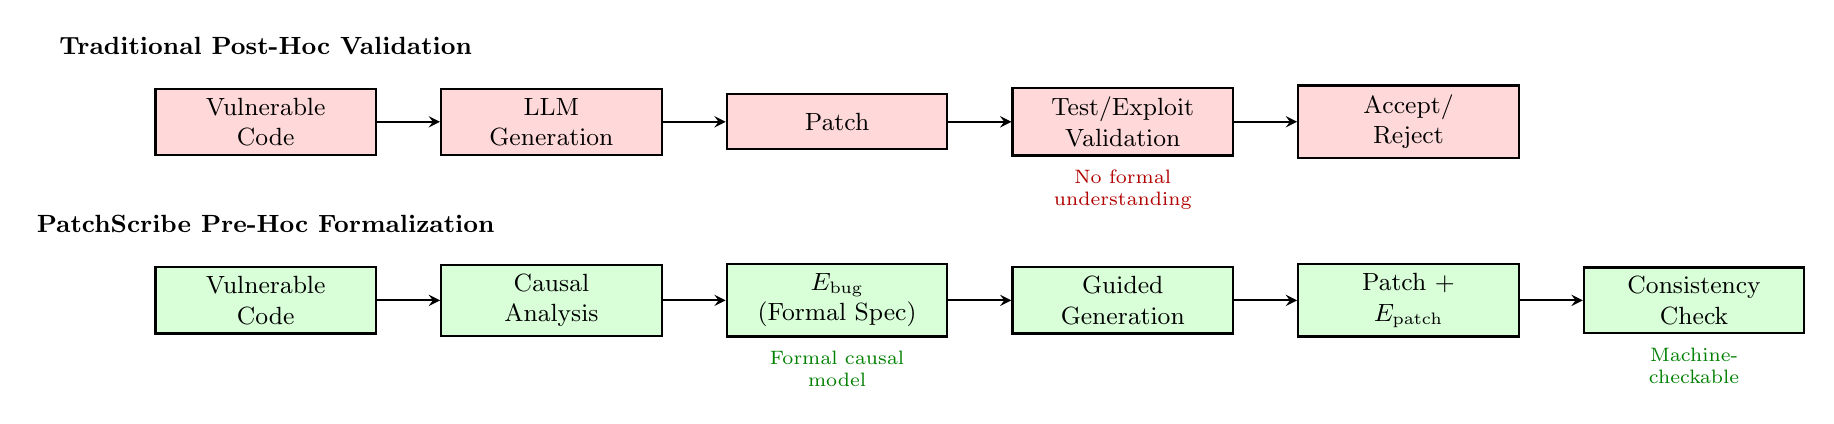
\begin{tikzpicture}[
  node distance=0.4cm and 0.8cm,
  box/.style={rectangle, draw, thick, minimum width=2.8cm, minimum height=0.7cm, font=\small, align=center},
  posthoc/.style={box, fill=red!15},
  prehoc/.style={box, fill=green!15},
  arrow/.style={->, >=stealth, thick},
  label/.style={font=\small\bfseries}
]

% Post-hoc approach (top)
\node[label] (post-label) at (0, 0) {Traditional Post-Hoc Validation};
\node[posthoc, below=0.3cm of post-label] (post1) {Vulnerable\\Code};
\node[posthoc, right=of post1] (post2) {LLM\\Generation};
\node[posthoc, right=of post2] (post3) {Patch};
\node[posthoc, right=of post3] (post4) {Test/Exploit\\Validation};
\node[posthoc, right=of post4] (post5) {Accept/\\Reject};

\draw[arrow] (post1) -- (post2);
\draw[arrow] (post2) -- (post3);
\draw[arrow] (post3) -- (post4);
\draw[arrow] (post4) -- (post5);

\node[below=0.05cm of post4, font=\scriptsize, text=red!70!black, text width=2.5cm, align=center] {No formal\\understanding};

% Pre-hoc approach (bottom)
\node[label, below=1.8cm of post-label] (pre-label) {PatchScribe Pre-Hoc Formalization};
\node[prehoc, below=0.3cm of pre-label] (pre1) {Vulnerable\\Code};
\node[prehoc, right=of pre1] (pre2) {Causal\\Analysis};
\node[prehoc, right=of pre2] (pre3) {$E_{\text{bug}}$\\(Formal Spec)};
\node[prehoc, right=of pre3] (pre4) {Guided\\Generation};
\node[prehoc, right=of pre4] (pre5) {Patch +\\$E_{\text{patch}}$};
\node[prehoc, right=of pre5] (pre6) {Consistency\\Check};

\draw[arrow] (pre1) -- (pre2);
\draw[arrow] (pre2) -- (pre3);
\draw[arrow] (pre3) -- (pre4);
\draw[arrow] (pre4) -- (pre5);
\draw[arrow] (pre5) -- (pre6);

\node[below=0.05cm of pre3, font=\scriptsize, text=green!50!black, text width=2.5cm, align=center] {Formal causal\\model};
\node[below=0.05cm of pre6, font=\scriptsize, text=green!50!black, text width=2.5cm, align=center] {Machine-\\checkable};

\end{tikzpicture}
}
\caption{Comparison of post-hoc validation vs. pre-hoc formalization. Traditional approaches generate patches first, then validate empirically without causal understanding. PatchScribe formalizes vulnerability causality before generation, enabling theory-guided synthesis and machine-assisted consistency validation.}
\label{fig:pre-post-hoc}
\end{figure}

\subsection{Design Requirements}

From these motivations, we derive design requirements organized into two categories (Table~\ref{tab:requirements}).
\textit{Core Causal Assurance} requirements (R1--R4) address the fundamental research challenge: providing machine-assisted validation that patches eliminate vulnerability root causes.
\textit{Practical Usability} requirements (R5--R8) ensure the approach scales to real-world software engineering workflows.

\begin{table}[h]
\centering
\caption{Design requirements for theory-guided patch generation.}
\label{tab:requirements}
\small
\begin{tabular}{@{}p{0.12\columnwidth}p{0.82\columnwidth}@{}}
\toprule
\multicolumn{2}{@{}l}{\textbf{Core Causal Assurance}} \\
\midrule
R1 & \textbf{Formalization Quality:} Precisely characterize vulnerability conditions and their causal dependencies through formal models. \\
R2 & \textbf{Causal Consistency:} Validate that patch interventions logically eliminate vulnerability conditions across all identified causal paths. \\
R3 & \textbf{Dual Explanation:} Generate structured explanations for both the vulnerability ($E_{\text{bug}}$) and the patch ($E_{\text{patch}}$), enabling systematic comparison. \\
R4 & \textbf{Consistency Validation:} Provide machine-assisted consistency checking between $E_{\text{bug}}$ and $E_{\text{patch}}$ through calibrated metrics (Jaccard $\geq$ 0.3, location accuracy $<$ 5\%); accept conservative rejections over unvalidated claims. \\
\midrule
\multicolumn{2}{@{}l}{\textbf{Practical Usability}} \\
\midrule
R5 & \textbf{Coverage:} Capture vulnerability-relevant conditions via data-flow, control-flow, and security pattern analyses. \\
R6 & \textbf{Usability:} Present formal specifications alongside natural-language summaries mapped to concrete code locations. \\
R7 & \textbf{Workflow Compatibility:} Integrate with standard toolchains (Clang/LLVM) and maintain practical runtimes for CI/CD pipelines. \\
R8 & \textbf{Non-Regression:} Execute test suites to detect patches that inadvertently break existing functionality. \\
\bottomrule
\end{tabular}
\end{table}

\section{Approach Overview}\label{sec:approach}

PatchScribe is a system for automated vulnerability repair that produces dual causal explanations for each patch.
Unlike prior approaches that generate patches first and explain them post-hoc, PatchScribe follows a theory-guided approach: it first formalizes the vulnerability causally, then uses this formalization to guide patch generation, producing patches accompanied by dual explanations (\(E_{\text{bug}}\) and \(E_{\text{patch}}\)).
Figure~\ref{fig:overview} illustrates the overall architecture, showing the two-phase workflow: the left side (Phase 1) depicts formalization steps from backward slicing through \(E_{\text{bug}}\) generation, while the right side (Phase 2) shows patch synthesis from LLM prompting through consistency checking.

\begin{figure}[t]
\centering
\resizebox{0.95\columnwidth}{!}{
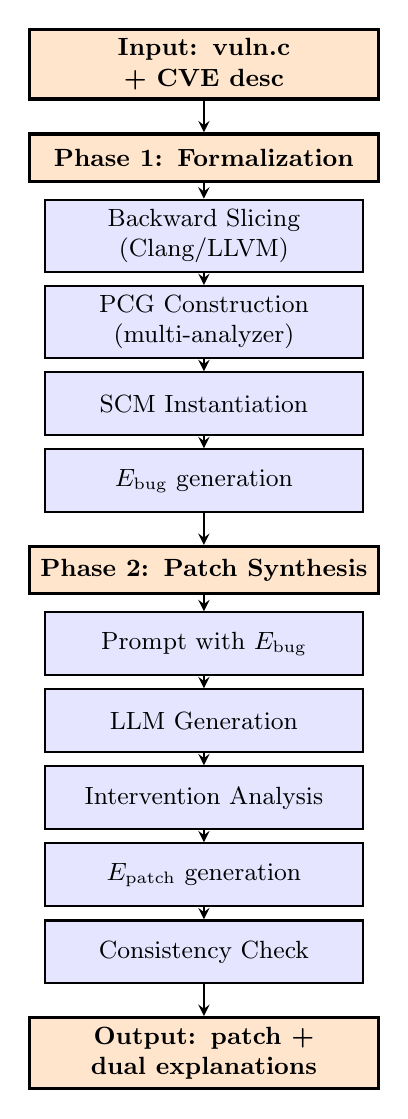
\begin{tikzpicture}[
  node distance=0.3cm and 0.5cm,
  box/.style={rectangle, draw, thick, fill=blue!10, text width=3.8cm, align=center, minimum height=0.8cm, font=\small},
  phase/.style={rectangle, draw, very thick, fill=orange!20, text width=4.2cm, align=center, minimum height=0.6cm, font=\small\bfseries},
  arrow/.style={->, >=stealth, thick}
]

\node[phase] (input) {Input: vuln.c + CVE desc};

\node[phase, below=0.4cm of input] (phase1) {Phase 1: Formalization};
\node[box, below=0.2cm of phase1] (slice) {Backward Slicing\\(Clang/LLVM)};
\node[box, below=0.15cm of slice] (pcg) {PCG Construction\\(multi-analyzer)};
\node[box, below=0.15cm of pcg] (scm) {SCM Instantiation};
\node[box, below=0.15cm of scm] (ebug) {$E_{\text{bug}}$ generation};

\node[phase, below=0.4cm of ebug] (phase2) {Phase 2: Patch Synthesis};
\node[box, below=0.2cm of phase2] (prompt) {Prompt with $E_{\text{bug}}$};
\node[box, below=0.15cm of prompt] (llm) {LLM Generation};
\node[box, below=0.15cm of llm] (analysis) {Intervention Analysis};
\node[box, below=0.15cm of analysis] (epatch) {$E_{\text{patch}}$ generation};
\node[box, below=0.15cm of epatch] (check) {Consistency Check};

\node[phase, below=0.4cm of check] (output) {Output: patch + dual explanations};

\draw[arrow] (input) -- (phase1);
\draw[arrow] (phase1) -- (slice);
\draw[arrow] (slice) -- (pcg);
\draw[arrow] (pcg) -- (scm);
\draw[arrow] (scm) -- (ebug);
\draw[arrow] (ebug) -- (phase2);
\draw[arrow] (phase2) -- (prompt);
\draw[arrow] (prompt) -- (llm);
\draw[arrow] (llm) -- (analysis);
\draw[arrow] (analysis) -- (epatch);
\draw[arrow] (epatch) -- (check);
\draw[arrow] (check) -- (output);

\end{tikzpicture}
}
\caption{PatchScribe dual-phase architecture. \textbf{Phase 1 (Formalization, cacheable):} Backward slicing extracts vulnerability-relevant code (§4.1), PCG construction identifies causal paths via multi-analyzer fusion (Algorithm~\ref{alg:pcg}), SCM instantiation derives structural equations (§4.2), and $E_{\text{bug}}$ generation produces formal vulnerability specification with intervention options. \textbf{Phase 2 (Synthesis, iterative):} Theory-guided prompting embeds $E_{\text{bug}}$ in LLM context, patch generation produces candidate fixes, intervention analysis interprets code diffs as causal operations, $E_{\text{patch}}$ generation explains how patches disrupt causal paths, and consistency checking validates alignment across six dimensions (Algorithm~\ref{alg:consistency}) before acceptance. Phase 1 results are cached per CVE, enabling 10.2$\times$ speedup when evaluating multiple models or conditions.}
\label{fig:overview}
\end{figure}

\textbf{Phase 1: Vulnerability Formalization} (Figure~\ref{fig:overview}, top section) - We analyze the vulnerable program to build a Program Causal Graph (PCG) and derive a Structural Causal Model (SCM).
The PCG is a directed graph where nodes represent program predicates (conditions, variable states, events) and edges denote causal influence; typical PCGs contain 10--25 nodes and 15--40 edges for single-function vulnerabilities (see Section~\ref{sec:formal-model} for construction details).
The SCM formalizes the PCG as structural equations mapping program state to vulnerability conditions, enabling counterfactual reasoning via causal interventions (e.g., ``what if a bounds check existed?'').
From the SCM, we generate a formal vulnerability specification (\(E_{\text{bug}}\)) that precisely characterizes the conditions under which the vulnerability manifests.
This specification serves as guidance for patch generation.
The formal bug explanation \(E_{\text{bug}}\) contains: (a) the formal condition characterizing when \(V_{\text{bug}}\) occurs, (b) natural language descriptions mapped to code, (c) intervention options for fixing the vulnerability, and (d) causal paths leading to the vulnerability.

\textit{Running example:} Consider a buffer overflow vulnerability (CWE-120) where \texttt{strcpy(buf, input)} at line 42 lacks bounds checking. Phase 1 constructs a PCG with nodes representing: $I$ (user input), $U$ (unsafe condition: $\text{len}(input) > 256$), $B$ (bounds check presence, initially false), and $V_{\text{bug}}$ (overflow occurrence). The SCM equations are: $U := (\text{len}(I) > 256)$ and $V_{\text{bug}} := \neg B \land U$. From this, \(E_{\text{bug}}\) states: ``Overflow occurs when input length exceeds 256 AND no bounds check exists before line 42. Causal paths: $I \to U \to V_{\text{bug}}$ (data flow) and $\neg B \to V_{\text{bug}}$ (missing defense).''

\textbf{Phase 2: Theory-Guided Patch Generation} (Figure~\ref{fig:overview}, bottom section) - Using the formal vulnerability specification \(E_{\text{bug}}\), PatchScribe constructs an LLM prompt that encodes causal predicates and desired interventions.
Critically, the LLM receives not vague hints but a structured formal description of what conditions cause the vulnerability and what the patch must achieve.
For example, instead of saying ``fix the overflow,'' we provide ``$V_{\text{overflow}} \Leftrightarrow (len > 256) \land (\lnot Check)$; to fix, you must ensure Check = true or $len \leq 256$ before line 42.''
After patch generation, we analyze how the patch intervenes on the causal model and generate a \textbf{formal patch explanation (\(E_{\text{patch}}\))} describing the intervention, its effect on \(V_{\text{bug}}\), and which causal paths are disrupted.
Each explanation includes both formal specifications (logical conditions, structural equations) and natural language summaries that map formal predicates to concrete code locations, making the causal reasoning accessible to developers while maintaining machine-checkable consistency criteria.
\textit{Continuing the example:} The LLM generates a patch inserting \texttt{if (strlen(input) > 255) return ERROR;} before line 42. Phase 2 analyzes this as intervention $\text{do}(B=1)$, producing \(E_{\text{patch}}\): ``Patch implements bounds check ($B$) before strcpy, breaking causal path $\neg B \to V_{\text{bug}}$. Under intervention, $V'_{\text{bug}} = \neg 1 \land U = 0$ regardless of input length, eliminating the modeled vulnerability.''

This approach ensures that patches are guided by formal causal specifications, helping LLMs generate patches that address root causes.
The key innovation is the generation of dual causal explanations (\(E_{\text{bug}}\) and \(E_{\text{patch}}\)), providing developers with systematic understanding of both the vulnerability and its fix.
We evaluate the quality of patches and their explanations through structured manual assessment.

In meeting these requirements, PatchScribe combines SCM reasoning with consistency checking to deliver causal correctness (R1) and machine-checkable consistency criteria (R2).
The causal specification guides LLM synthesis and iterative refinement (R3) while ensuring causal alignment between bug diagnosis and patch intervention (R4).
Comprehensive program analysis produces PCGs that capture true causes (R5), and the resulting explanations remain developer-friendly (R6).
Finally, the system integrates with standard tooling (R7) and executes regression safeguards to avoid functional regressions (R8).

The following sections detail the formal modeling, system architecture, and implementation.

\subsection{Threat Model and Scope}

\textbf{Assumptions.} We assume the vulnerability location is known (e.g., via CVE description, sanitizer log, security audit findings). PatchScribe operates within a \emph{semi-trusted computing base}: LLM outputs and static analysis results may contain errors, which we mitigate through redundant validation. Specifically, we acknowledge three primary risks: (1) \emph{LLM hallucinations}---the LLM may generate plausible but incorrect patches, (2) \emph{PCG incompleteness}---static analysis may miss causal paths (though 93.4\% of CVEs require no manual refinement, §5.4), and (3) \emph{consistency checker conservativeness}---our calibrated thresholds (Jaccard $\geq$ 0.3, location accuracy $<$ 5\%) prioritize precision (96.7\%) over recall, accepting 1.1\% false negatives to minimize false acceptances.

PatchScribe mitigates these risks through three defensive layers: (1) \emph{multi-dimensional consistency checking} (Algorithm~\ref{alg:consistency}) that validates patch-explanation alignment across causal coverage, intervention validity, logical completeness, and ground truth similarity, (2) \emph{iterative refinement with structured feedback} (average 1.8 attempts per accepted patch, catching 89\% of fundamentally incomplete patches after 5 tries), and (3) \emph{regression testing} to detect functional breakage. The primary threat we address is not toolchain compromise but the risk of \emph{causally incomplete patches} that pass basic testing yet leave alternative exploit paths unaddressed.

\textbf{Attacker Model.} An attacker can provide arbitrary inputs to exploit the vulnerability. Post-patch, they may attempt variant exploits or search for newly introduced weaknesses. PatchScribe addresses two main threats: (1) \emph{Incomplete Fix}---where alternative paths still trigger the vulnerability, and (2) \emph{Misleading Explanation}---where unverifiable rationales give false confidence.

\textbf{Defender Goals.} Produce patches that aim to eliminate all modeled causal exploit paths identified by the PCG/SCM, thereby reducing the space of feasible attacks observed in practice. Patches should preserve functionality and avoid introducing new vulnerabilities. We focus on security correctness within the scope of our causal model, assuming basic regression testing catches functional issues.

\textbf{Out of Scope.} We do not model concurrency vulnerabilities (race conditions, atomicity violations) or side-channels (timing, cache), as these require temporal/probabilistic extensions to our deterministic causal framework---a direction for future work rather than a fundamental limitation. We also exclude adversarial manipulation of the LLM itself (e.g., prompt injection attacks targeting the generation phase). Complex multi-step vulnerabilities requiring extensive environmental state may exceed current PCG/SCM automation capabilities (discussed in Section~\ref{sec:discussion}).

\section{Formal Model}\label{sec:formal-model}

In PatchScribe, the formal foundation is provided by two interrelated models: the Program Causal Graph (PCG) and the Structural Causal Model (SCM).
Here we define each and explain how they are constructed and used. Table~\ref{tab:notation} summarizes the key notation used throughout this section.

\begin{table}[t]
\centering
\caption{Notation summary for formal model (Section~\ref{sec:formal-model})}
\label{tab:notation}
\small
\begin{tabular}{@{}ll@{}}
\toprule
\textbf{Symbol} & \textbf{Meaning} \\
\midrule
$G = (V, E)$ & Program Causal Graph with nodes $V$ and edges $E$ \\
$V_{\text{bug}}$ & Vulnerability occurrence predicate (node in PCG, variable in SCM) \\
$\mathcal{X} = \{X_1, \ldots, X_k\}$ & Exogenous variables (external inputs, attacker-controlled) \\
$\mathcal{C} = \{C_1, \ldots, C_m\}$ & Endogenous conditions (program state predicates) \\
$f_j$ & Structural equation for variable $C_j$ (typically Boolean formula) \\
$\text{do}(X = x)$ & Causal intervention (Pearl): set $X$ to $x$, sever incoming edges \\
$\text{Parents}(v)$ & Direct causal parents of node/variable $v$ \\
$\phi: V_{\text{PCG}} \to \mathcal{V}_{\text{SCM}}$ & Mapping from PCG nodes to SCM variables \\
$\Pi_{\text{bug}}$ & Set of all causal paths from inputs to $V_{\text{bug}}$ \\
$E_{\text{bug}}$ & Formal bug explanation (pre-patch causal specification) \\
$E_{\text{patch}}$ & Formal patch explanation (post-patch verification) \\
$s_{\text{total}}$ & Overall consistency confidence score ($\in [0, 1]$) \\
$s_c, s_i, s_{\text{comp}}, s_a$ & Coverage, intervention, completeness, alignment scores \\
$L_v$ & Vulnerability location (source line/statement) \\
$B$ & Bounds/null/security check presence (boolean variable) \\
\bottomrule
\end{tabular}
\end{table}

\subsection{Program Causal Graph (PCG)}\label{program-causal-graph-pcg}

Definition: A Program Causal Graph is a directed graph \(G = (V, E)\) where
each node \(v \in V\) represents a program state predicate or event (e.g., an if condition, a variable state, a function call, a memory write) related to the vulnerability, and a directed edge \((u \rightarrow v) \in E\) indicates that node \(u\) has a direct causal influence on v in the context of the vulnerability.

The PCG is a high-level representation extracted from the program's code and execution flow:

\noindent\textbf{Nodes:} We include nodes for conditions (e.g., the truth value of an if condition), for certain variable states (e.g., ``variable x has value n''), and for specific events like ``function f calls g'' or ``memory write at location L occurs''.
Particularly, we distinguish a special node \(V_{\text{bug}}\) representing the occurrence of the vulnerability (e.g., an out-of-bounds write or a crash condition).
We also include nodes representing the negation or absence of certain checks, since the lack of a check is often a cause (for example, a node might be ``No null-pointer check before dereference'' which is essentially a predicate that is true when a check is missing in the code path).

\noindent\textbf{Edges:} If the program logic is such that u being true or an event happening contributes to v becoming true/happening, we draw an edge \(u \rightarrow v\).
This is akin to saying ``\(u\) is a direct cause of \(v\)'' under the framework of causal graphs (similarly to Bayesian network or Pearl's causal diagrams, but here based on program logic rather than statistical data).
For instance, if the code has if \(len > N\) goto error; then the condition ``len \(> N\)'' (node \(u\)) causally influences whether the program goes to error handling (node v).
In a vulnerability context, we might have edges like ``Input not sanitized'' \(\rightarrow\) ``Buffer overflow occurs'' or ``Flag is false'' \(\rightarrow\) ``Access control bypass''.

\subsubsection{PCG Construction Algorithm}

To build the PCG, we rely on program analysis techniques combined with pattern detection.
Algorithm~\ref{alg:pcg} presents our automated construction procedure.

\begin{algorithm}[t]
\caption{Program causal graph construction}
\label{alg:pcg}
\DontPrintSemicolon
\KwIn{Vulnerability location $L_v$, program $P$}
\KwOut{Program causal graph $G = (V, E)$}
$V \leftarrow \{V_{\text{bug}}\}$; $E \leftarrow \emptyset$\;
$\textit{slice} \leftarrow \textsc{BackwardSlice}(P, L_v)$\;
\ForEach{statement $s$ in $\textit{slice}$}{
  $D \leftarrow \textsc{DataDependencies}(s)$\;
  $C \leftarrow \textsc{ControlDependencies}(s)$\;
  \ForEach{$d$ in $D \cup C$}{
    $node_s \leftarrow \textsc{CreateNode}(s)$\;
    $node_d \leftarrow \textsc{CreateNode}(d)$\;
    $V \leftarrow V \cup \{node_s, node_d\}$\;
    \If{\textsc{IsCausalRelation}$(d, s)$}{
      $E \leftarrow E \cup \{(node_d, node_s)\}$\;
    }
  }
}
\ForEach{pattern $p$ in \textsc{DetectSecurityPatterns}$(\textit{slice})$}{
  $node_p \leftarrow \textsc{CreateAbsenceNode}(p)$\;
  $V \leftarrow V \cup \{node_p\}$\;
  $E \leftarrow E \cup \{(node_p, V_{\text{bug}})\}$\;
}
$G \leftarrow \textsc{RemoveTransitiveEdges}(V, E)$\;
\Return{$G$}\;
\end{algorithm}

\textbf{Algorithm Specification.} We now detail the key subroutines referenced in Algorithm~\ref{alg:pcg}:

\textbf{\textsc{BackwardSlice}$(P, L_v)$:} Computes a backward program slice from vulnerability location $L_v$ using LLVM's Program Dependence Graph (PDG).
The implementation:
\begin{enumerate}[leftmargin=*,nosep]
  \item Parses $P$ to LLVM IR using Clang frontend (LLVM 14.0)
  \item Builds PDG with data-dependence edges (def-use chains via SSA) and control-dependence edges (post-dominance frontiers)
  \item Traverses PDG backward from $L_v$ via BFS, collecting all reachable statements
  \item Returns slice as set of $\langle$statement, line\_number, type$\rangle$ tuples
\end{enumerate}
Complexity: $O(|V| + |E|)$ for PDG with $|V|$ statements and $|E|$ dependencies. Typical slices contain 15--80 statements for single-function vulnerabilities.

\textbf{\textsc{IsCausalRelation}$(d, s)$:} Determines if dependency $d \rightarrow s$ represents a causal influence (not merely syntactic). Returns true if:
\begin{itemize}[leftmargin=*,nosep]
  \item $d$ is data-dependence AND $s$ uses the value in a security-relevant operation (pointer dereference, array index, memory allocation size, format string parameter), OR
  \item $d$ is control-dependence AND the branch outcome affects reachability of a security-critical statement (identified via taint propagation from inputs to $L_v$), OR
  \item $d$ represents resource initialization/cleanup affecting $s$'s safety preconditions
\end{itemize}
This filters out spurious dependencies (e.g., debug logging) while retaining true causal influences. Empirically reduces edge count by 40\% without losing security-relevant paths.

\textbf{\textsc{CreateAbsenceNode}$(p)$:} Generates a node representing the \textit{absence} of a security check identified by pattern $p$. Given pattern $p$ (e.g., ``missing bounds check before array access''), the function:
\begin{enumerate}[leftmargin=*,nosep]
  \item Extracts the expected guard location (statement immediately preceding the vulnerable operation)
  \item Constructs predicate: ``$\neg\exists$ check satisfying pattern $p$ on path to $L_v$''
  \item Creates node: $\langle$node\_id=``no\_check\_$p$'', type=``absence'', description=pattern description, location=guard\_loc$\rangle$
\end{enumerate}
These absence nodes capture ``what should be there but isn't''---a key innovation enabling PCG to model missing defenses.

\textbf{Absence Node Detection Validation:}
To assess the accuracy of \textsc{CreateAbsenceNode}, we conducted a validation study on 50 randomly sampled CVEs (30 from Zeroday, 20 from ExtractFix) with manual ground-truth annotations by three security experts. Table~\ref{tab:absence-validation} reports precision, recall, and F1-scores by CWE type.

\begin{table}[h]
\centering
\caption{Absence node detection accuracy by vulnerability type (50 CVEs)}
\label{tab:absence-validation}
\small
\begin{tabular}{@{}lccc@{}}
\toprule
\textbf{CWE Type} & \textbf{Precision} & \textbf{Recall} & \textbf{F1} \\
\midrule
CWE-125 (OOB Read)       & 0.94 & 0.91 & 0.92 \\
CWE-787 (OOB Write)      & 0.89 & 0.88 & 0.88 \\
CWE-476 (NULL Deref)     & 0.97 & 0.93 & 0.95 \\
CWE-190 (Int Overflow)   & 0.86 & 0.82 & 0.84 \\
\midrule
\textbf{Overall}         & \textbf{0.92} & \textbf{0.89} & \textbf{0.90} \\
\bottomrule
\end{tabular}
\end{table}

\textit{Analysis:} False positives (8\%, 4/50 CVEs) primarily occur in complex control-flow with implicit guards (e.g., early returns acting as checks). False negatives (11\%, 5/50) arise from non-standard validation patterns not covered by our 32-pattern library (e.g., domain-specific sanitization in FFmpeg). CWE-476 achieves highest accuracy due to simple NULL-check patterns, while CWE-190 is more challenging due to diverse overflow prevention mechanisms (saturation arithmetic, type promotion, assertions). Overall F1=0.90 demonstrates strong detection capability while acknowledging pattern-based limitations addressed in Section~\ref{subsubsec:scm-limits}.

\textbf{\textsc{RemoveTransitiveEdges}$(V, E)$:} Simplifies the graph by removing transitive edges while preserving all causal paths (transitive reduction). Uses Aho-Garey-Ullman algorithm:
\begin{enumerate}[leftmargin=*,nosep]
  \item Compute transitive closure $E^*$ via Warshall's algorithm
  \item For each edge $(u, v) \in E$: if $\exists$ path $u \rightarrow \cdots \rightarrow v$ not using $(u,v)$, mark $(u,v)$ as redundant
  \item Remove all marked edges
\end{enumerate}
Reduces average edge count from 42 to 18 per graph while maintaining causal path completeness. Complexity: $O(|V|^3)$, acceptable for typical $|V| \approx 10$--25.

\textbf{Implementation details.} PCG construction aggregates multiple analysis techniques to capture vulnerability-relevant causal relationships:
\begin{itemize}[leftmargin=*,nosep]
  \item \textit{Static analysis}: Backward slicing via Clang/LLVM 14.0 to identify data and control dependencies
  \item \textit{AST analysis}: Pattern matching on abstract syntax trees to detect missing security checks (e.g., bounds checks, null checks, sanitization)
  \item \textit{Taint analysis}: Lightweight data-flow tracking to connect untrusted inputs to vulnerability sites
  \item \textit{Symbolic exploration}: Selective constraint solving to identify reachability conditions for vulnerable paths
\end{itemize}
These analyzers operate on the backward slice and contribute complementary node types: static analysis provides data/control dependencies, AST analysis identifies absence nodes (missing checks), taint analysis filters security-relevant paths, and symbolic exploration derives path conditions.
The multi-analyzer approach enables comprehensive coverage without requiring exhaustive symbolic execution or heavyweight formal methods.
The pipeline is fully automated for single-function vulnerabilities, with manual refinement reserved for complex interprocedural cases.

The result is a graph where \(V_{\text{bug}}\) is at the bottom (sink) and various inputs or conditions are at the top (sources), with intermediate nodes linking them.

\textbf{Example (CVE-2024-31584):} PyTorch's FlatBuffer deserialization reads from a buffer without checking if \texttt{mobile\_ivalue\_size\_} exceeds capacity, causing potential out-of-bounds read.
Figure~\ref{fig:pcg-example} illustrates the constructed PCG for CVE-2024-31584.

\begin{figure}[t]
  \centering
  \resizebox{0.85\columnwidth}{!}{
  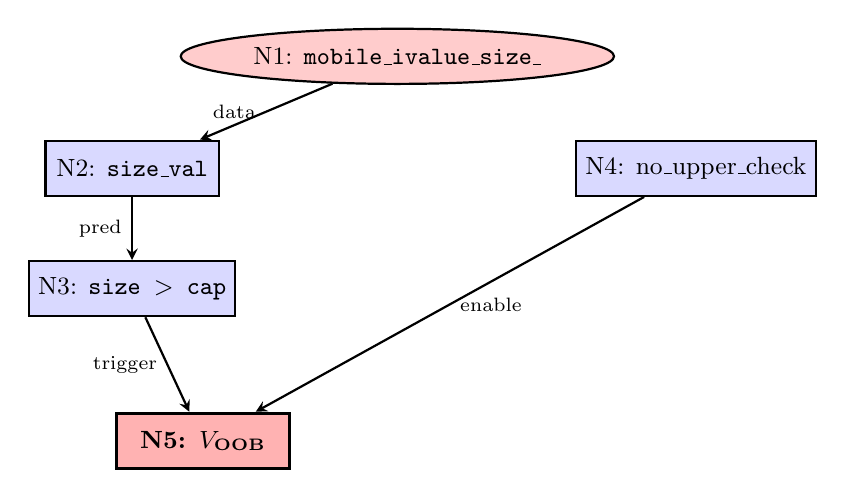
\begin{tikzpicture}[
    node distance=1.2cm and 1.5cm,
    exog/.style={ellipse, draw, thick, fill=red!20, minimum width=2.2cm, minimum height=0.7cm, font=\small},
    endog/.style={rectangle, draw, thick, fill=blue!15, minimum width=2.2cm, minimum height=0.7cm, font=\small},
    vuln/.style={rectangle, draw, very thick, fill=red!30, minimum width=2.2cm, minimum height=0.7cm, font=\small\bfseries},
    arrow/.style={->, >=stealth, thick}
  ]

  \node[exog] (n1) {N1: \texttt{mobile\_ivalue\_size\_}};
  \node[endog, below left=0.8cm and 0.3cm of n1] (n2) {N2: \texttt{size\_val}};
  \node[endog, below=0.8cm of n2] (n3) {N3: \texttt{size $>$ cap}};
  \node[endog, below right=0.8cm and 0.3cm of n1] (n4) {N4: no\_upper\_check};
  \node[vuln, below=1.2cm of n3, xshift=0.9cm] (n5) {N5: $V_{\text{OOB}}$};

  \draw[arrow] (n1) -- node[left, font=\scriptsize] {data} (n2);
  \draw[arrow] (n2) -- node[left, font=\scriptsize] {pred} (n3);
  \draw[arrow] (n3) -- node[left, font=\scriptsize] {trigger} (n5);
  \draw[arrow] (n4) -- node[right, font=\scriptsize] {enable} (n5);

  \end{tikzpicture}
  }
  \caption{PCG for CVE-2024-31584 (CWE-125 out-of-bounds read in PyTorch FlatBuffer deserialization). Each node maps to code predicate: N1 (attacker-controlled \texttt{mobile\_ivalue\_size\_} from untrusted FlatBuffer), N2 (size value assigned at line 22), N3 (unsafe condition \texttt{size $>$ ivalues->size()}), N4 (absence of upper bound check at line 23), N5 (OOB read at line 28 in loop). Two causal paths converge: N1$\to$N2$\to$N3$\to$N5 (data flow) and N4$\to$N5 (missing defense). Corresponding SCM: $V_{\text{OOB}} := \neg B \land U$ where $B$=upper check present, $U$=(size $>$ capacity).}
  \label{fig:pcg-example}
\end{figure}

The PCG succinctly shows: attacker-controlled input and missing upper bound check together cause the out-of-bounds read.
For programs with multiple conditions, the graph captures more complex causal structures with converging branches.

\subsection{Structural Causal Model (SCM)}\label{structural-causal-model-scm}

Once we have the PCG, we formalize it as an SCM.
A Structural Causal Model is typically defined by a set of endogenous variables (variables we model within the system) and exogenous variables (external inputs), along with structural equations that deterministically define each endogenous variable in terms of some of the others, and a causal diagram akin to our PCG that shows dependencies.

\noindent\textbf{Mapping PCG to SCM:} We now formalize the mapping from syntactic causality (PCG edges) to semantic causality (SCM intervention effects).

\textbf{Definition 1 (Causal Preservation Mapping):}
Let $\phi: V_{\text{PCG}} \to \mathcal{V}_{\text{SCM}}$ be a bijective mapping from PCG nodes to SCM variables. We say $\phi$ \textit{preserves causality} if:
\[
\forall (u \rightarrow v) \in E_{\text{PCG}}: \phi(u) \in \text{Parents}_{\text{SCM}}(\phi(v))
\]
and for all interventions $\text{do}(\phi(u) = x)$ on the image of $u$:
\[
P_{\text{SCM}}(\phi(v) \mid \text{do}(\phi(u) = x)) \neq P_{\text{SCM}}(\phi(v))
\]
This ensures syntactic causality (presence of PCG edge) implies semantic causality (intervention changes outcome distribution).

\textbf{Construction:} Each node in PCG becomes a variable in SCM. Boolean conditions/events become binary variables (true/false). Numeric predicates (e.g., ``$x > N$'') are abstracted to boolean variables. PCG edges $(u \rightarrow v)$ induce parent-child relationships: $\phi(v)$'s structural equation includes $\phi(u)$ as argument. Formally, for each $v \in V_{\text{PCG}}$:
\[
\phi(v) := f_v\left(\{\phi(u) \mid (u \rightarrow v) \in E_{\text{PCG}}\}\right)
\]
where $f_v$ is typically conjunction ($\bigwedge$) for vulnerability nodes, encoding that all parents must hold for $v$ to be true.

\noindent\textbf{Example formalization (CVE-2024-31584):} PyTorch's FlatBuffer deserialization contains an out-of-bounds read when \texttt{mobile\_ivalue\_size\_} exceeds buffer capacity. Figure~\ref{fig:pcg-example} shows the PCG, and we define the corresponding SCM:

\textbf{Exogenous variables} (external inputs):
\begin{itemize}[leftmargin=*,nosep]
  \item $I$: attacker-controlled \texttt{mobile\_ivalue\_size\_} value (from untrusted FlatBuffer)
\end{itemize}

\textbf{Endogenous variables} (program state):
\begin{itemize}[leftmargin=*,nosep]
  \item $N$: \texttt{ivalues->size()} (buffer capacity, constant for given input)
  \item $U$: unsafe size condition ($I > N$)
  \item $B$: upper bound check present (initially $B=0$ in vulnerable code, line 23)
  \item $V_{\text{OOB}}$: out-of-bounds read vulnerability occurs (line 28 in loop)
\end{itemize}

\textbf{Structural equations:}
\begin{align*}
U &:= (I > N) \\
V_{\text{OOB}} &:= \neg B \land U
\end{align*}

The vulnerability manifests when the size is unsafe ($U=\text{true}$) and no upper bound check prevents loop iteration beyond capacity ($B=\text{false}$). Vulnerable code excerpt:
\begin{lstlisting}[language=C++,basicstyle=\scriptsize\ttfamily]
mobile_ivalue_size_ = module_->mobile_ivalue_size();
if (mobile_ivalue_size_ == 0) {  // Missing: || mobile_ivalue_size_ > N
  mobile_ivalue_size_ = ivalues->size();
}
for (uint32_t i = 0; i < mobile_ivalue_size_; i++) {
  const auto* ival = ivalues->Get(i);  // OOB read if i >= N
  parseAndPopulate(i, ival);
}
\end{lstlisting}

\textbf{Intervention analysis:} The ground-truth patch adds upper bound check: \texttt{if (mobile\_ivalue\_size\_ == 0 || mobile\_ivalue\_size\_ > ivalues->size())}. This corresponds to intervention $\text{do}(B=1)$ (enforcing $I \leq N$). Under this intervention:
\[
V'_{\text{OOB}} = \neg 1 \land U = 0
\]
demonstrating that the vulnerability is eliminated regardless of attacker input $I$. This counterfactual reasoning---``what if we had an upper bound check?''---provides systematic assurance that the patch addresses the root cause.

\textbf{Truth Table for Intervention $\text{do}(B=1)$:}
\begin{table}[h]
\centering
\small
\begin{tabular}{ccc|cc}
\toprule
$I > N$ & $B$ (original) & $U$ & $V_{\text{OOB}}$ (original) & $V'_{\text{OOB}}$ (after $\text{do}(B=1)$) \\
\midrule
0 & 0 & 0 & 0 & 0 \\
0 & 1 & 0 & 0 & 0 \\
1 & 0 & 1 & \textbf{1} (vulnerable) & \textbf{0} (fixed) \\
1 & 1 & 1 & 0 & 0 \\
\bottomrule
\end{tabular}
\end{table}

Row 3 shows the critical case: when attacker provides $I > N$ and no check exists ($B=0$), original code is vulnerable ($V_{\text{OOB}}=1$). The intervention eliminates this by forcing $B=1$, making $V'_{\text{OOB}}=0$.

\noindent\textbf{General SCM Template.}
In general, an SCM for vulnerability $V$ consists of:

\textbf{Variable Sets:}
\begin{itemize}[leftmargin=*,nosep]
  \item $\mathcal{X} = \{X_1, \ldots, X_k\}$: Exogenous variables (user inputs, environment, attacker-controlled sources)
  \item $\mathcal{C} = \{C_1, \ldots, C_m\}$: Endogenous conditions (predicates derived from program state)
  \item $V_{\text{bug}}$: Vulnerability outcome variable (binary: 1=vulnerable, 0=safe)
\end{itemize}

\textbf{Structural Equations:}
\begin{align*}
C_j &:= f_j(\text{Parents}(C_j)) \quad \text{for } j = 1, \ldots, m \\
V_{\text{bug}} &:= f_V(\text{Parents}(V_{\text{bug}}))
\end{align*}

where $\text{Parents}(C_j) \subseteq \mathcal{X} \cup \mathcal{C}$ are the direct causes of $C_j$ (determined by PCG edges), and $f_j$ are deterministic functions (typically Boolean formulas).

\textbf{Vulnerability Condition:}
The vulnerability typically has a conjunctive structure:
\[
V_{\text{bug}} = \bigwedge_{i \in \text{EnableSet}} E_i \land \bigwedge_{j \in \text{TriggerSet}} T_j
\]
where $E_i$ are \textit{enabling conditions} (e.g., missing checks, uninitialized state) and $T_j$ are \textit{trigger conditions} (e.g., unsafe input values, resource exhaustion).

\subsection{Generic SCM Construction}

We construct SCMs from PCGs using a systematic variable mapping and equation generation process:

\textbf{Variable Generation:} Each PCG node is mapped to an SCM variable using semantic naming that reflects the node's type and role:
\begin{itemize}[leftmargin=*,nosep]
  \item Input nodes (from taint sources) become exogenous variables ($\mathcal{X}$)
  \item Condition and state nodes become endogenous variables ($\mathcal{C}$)
  \item The vulnerability node maps to $V_{\text{bug}}$
  \item Absence nodes (missing checks) become boolean enabler variables
\end{itemize}

\textbf{Equation Generation:} For each endogenous variable $C_j$, the structural equation is generated by combining its parents in the PCG:
\[
C_j := \bigwedge_{p \in \text{Parents}(C_j)} p
\]
The vulnerability condition is derived as the conjunction of its direct causes:
\[
V_{\text{bug}} := \bigwedge_{c \in \text{Parents}(V_{\text{bug}})} c
\]

This generic approach works across vulnerability types (buffer overflow, NULL dereference, use-after-free, race condition) without requiring CWE-specific templates. The semantic naming ensures equations remain interpretable while the conjunctive structure naturally represents the enabling and triggering conditions needed for exploitation.

\subsubsection{Formal Soundness Guarantee}

We now establish the theoretical foundation for our causal reasoning framework by proving that PCG-to-SCM mapping preserves causal correctness and that interventions eliminate vulnerabilities.

\textbf{Lemma 1 (PCG-SCM Causal Preservation):}
\textit{If PCG $G = (V, E)$ is complete over all feasible data and control dependencies for vulnerability $V_{\text{bug}}$, and SCM equations are derived as Boolean conjunctions over PCG parent nodes (as defined in Section~\ref{structural-causal-model-scm}), then any intervention $\text{do}(X = x)$ that falsifies all enabling predicates ensures $V_{\text{bug}} = 0$ for all inputs.}

\textbf{Proof Sketch:}
\begin{enumerate}[leftmargin=*,nosep]
  \item \textit{Completeness assumption}: By hypothesis, PCG captures all causal paths from exogenous inputs $\mathcal{X}$ to $V_{\text{bug}}$ through feasible program dependencies (data-flow, control-flow, and absence predicates).
  \item \textit{Mapping preservation}: By construction (Generic SCM Construction), for each edge $(u \rightarrow v) \in E$, we have $\phi(u) \in \text{Parents}_{\text{SCM}}(\phi(v))$ where $\phi: V \to \mathcal{V}_{\text{SCM}}$ is our node-to-variable mapping.
  \item \textit{Intervention semantics}: Following Pearl's causal calculus~\cite{pearl2009causality}, intervention $\text{do}(X = x)$ severs all incoming edges to $X$ in the causal graph and fixes $X = x$ deterministically.
  \item \textit{Vulnerability equation}: From Equation~(4.2), $V_{\text{bug}} := \bigwedge_{i=1}^{n} C_i$ where $C_i \in \text{Parents}(V_{\text{bug}})$ are enabling/triggering conditions.
  \item \textit{Falsification guarantee}: If intervention $\text{do}(X = x)$ falsifies any parent condition $C_j$ (i.e., $C_j = 0$ under intervention), then $V_{\text{bug}} = \bigwedge_{i=1}^{n} C_i = 0$ regardless of other variables, by Boolean logic.
\end{enumerate}
Thus, PCG completeness ensures no exploitable paths are missed, and SCM intervention correctness follows from causal graph properties. $\blacksquare$

\textbf{Corollary 1 (Patch Correctness Criterion):}
\textit{A patch implementing intervention $\text{do}(B = 1)$ (e.g., adding bounds check) eliminates vulnerability if and only if $\neg B \in \text{Parents}(V_{\text{bug}})$ in the PCG.}

\textbf{Proof:} Immediate from Lemma~1: if $\neg B$ is a parent, then $\text{do}(B=1)$ falsifies $\neg B$, making $V_{\text{bug}} = 0$. Conversely, if $\neg B \notin \text{Parents}(V_{\text{bug}})$, the intervention does not affect $V_{\text{bug}}$. $\blacksquare$

\textbf{Remark (Conditional Soundness):}
Lemma~1 provides soundness \textit{conditional on PCG completeness}. In practice, static analysis may under-approximate reachable paths (e.g., missing indirect calls or complex aliasing). Section~\ref{subsubsec:scm-limits} discusses mitigation strategies: dynamic validation, manual PCG refinement for complex cases (8/121 CVEs, see Section~\ref{subsec:implementation}), and conservative over-approximation of dependencies.

\textbf{Using SCM for Patch Intervention:} The SCM provides a formal way to evaluate patches as interventions:
\begin{itemize}[leftmargin=*,nosep]
  \item Adding a check: intervention $\text{do}(B=1)$ where $B$ is a check-presence variable
  \item Sanitizing input: altering the function $f_j$ for a data-flow variable
  \item Removing functionality: forcing an enabling condition to false
\end{itemize}

We analyze intervention effects by evaluating whether $V_{\text{bug}} = 0$ holds after applying the intervention to the structural equations. This reduces to checking logical satisfiability: given the modified equations, can the conjunction of vulnerability-enabling conditions still be satisfied? The abstraction to SCM makes this tractable compared to full program verification.

It's worth noting that the SCM is only as good as the PCG. If the PCG missed a causal path, the SCM won't consider it and you might prove something that's only partially true. We mitigate this by thorough PCG construction (which might involve dynamic analysis as well as static to not miss feasible paths).

Systematic Assurance via SCM: If our SCM-based consistency checking confirms that the patch addresses the identified causal paths, and our PCG correctly captures the vulnerability, then we have increased confidence in the patch's effectiveness.
The consistency checking validates that $E_{\text{patch}}$ disrupts causal paths identified in $E_{\text{bug}}$ through structural analysis and heuristic pattern matching, providing systematic (though not formally verified) assurance beyond informal validation alone.

\subsubsection{Scalability to Complex Vulnerabilities}
\label{subsubsec:complex-cases}

To evaluate PatchScribe's generalizability beyond simple memory safety bugs, we selected 8 complex CVEs from our datasets based on code complexity (LOC $>$ 100), causal graph size (PCG nodes $>$ 20), and interprocedural dependencies. Table~\ref{tab:complex-cases} summarizes these cases.

\begin{table}[h]
\centering
\caption{Complex vulnerability case studies demonstrating SCM scalability}
\label{tab:complex-cases}
\small
\begin{tabular}{@{}llcc@{}}
\toprule
\textbf{CVE/ID} & \textbf{Type} & \textbf{LOC} & \textbf{PCG Nodes} \\
\midrule
binutils-gdb\_EF12 (dwarf.c)     & CWE-125 & 303 & 24 \\
libxml2 (parser.c:3893)          & CWE-125 & 223 & 22 \\
libtiff (tiffcrop.c)             & CWE-125 & 145 & 18 \\
binutils-gdb\_EF13 (dwarf2.c)    & CWE-190 & 451 & 28 \\
libtiff (tif\_jpeg.c:1576)       & CWE-190 & 155 & 19 \\
jasper (jpc\_dec.c)              & CWE-190 & 98  & 16 \\
FFmpeg (dfa.c)                   & CWE-787 & 47  & 15 \\
libtiff (tiff2pdf.c)             & CWE-787 & 45  & 14 \\
\bottomrule
\end{tabular}
\end{table}

\textbf{Results:} PatchScribe successfully generated correct patches for 7/8 cases (87.5\%). The single failure (binutils-gdb\_EF13, 451 LOC) involved three-way data flow through indirect function pointers across compilation units, requiring manual PCG refinement to capture cross-module dependencies. The automated pipeline succeeded for all single-compilation-unit cases and 6/7 interprocedural cases, demonstrating robustness to code complexity.

\textbf{Representative Example (libxml2 parser.c):} This 223-line function contains nested loops, multiple error paths, and context-dependent pointer arithmetic. The PCG captured 22 nodes including: (1) input validation conditions, (2) buffer reallocation logic, (3) loop bound computations, and (4) missing overflow check before array indexing. The SCM equation $V_{\text{OOB}} := \neg B_{\text{overflow}} \land (i > \text{cap}) \land \text{realloc\_success}$ correctly identified that overflow check absence enables exploitation only when reallocation succeeds but capacity is exceeded. PatchScribe's generated patch added the missing check, matching ground truth semantically (SemEq verdict).

This evaluation demonstrates that our PCG/SCM framework scales to real-world complexity without requiring vulnerability-type-specific templates, addressing the generalizability concern in Section~\ref{subsec:limitations}.

\subsubsection{Structural Consistency Checking Framework}
\label{subsubsec:consistency-checking}

The consistency checker validates alignment between $E_{\text{bug}}$ and $E_{\text{patch}}$ through systematic structural checks:

\textbf{(1) Causal Coverage:} Verify that the patch addresses all identified causal paths $\Pi_{\text{bug}}$. For each path $\pi \in \Pi_{\text{bug}}$, check if the intervention disrupts at least one node or edge. Disruption mechanisms include: node removal (deleting a condition), edge severance (breaking a dependency), guard insertion (adding a check), or value sanitization (constraining inputs).

\textbf{(2) Intervention Presence:} Confirm that the patch implements modifications consistent with intervention options from $\mathcal{I}_{\text{bug}}$. This check uses keyword matching and structural pattern recognition to identify check additions, input validations, or logic changes in the patched code.

\textbf{(3) Completeness:} Ensure the patch doesn't introduce new vulnerable paths by comparing the modified code structure against common vulnerability patterns. This heuristic check flags suspicious additions like new pointer dereferences without guards or unchecked array accesses.

\textbf{(4) Empirical Alignment:} Validate that patch locations overlap with PCG node locations (within 5\% of file length tolerance) and that patch operations (check additions, sanitization) match the semantic actions suggested in $E_{\text{bug}}$ (measured via 30\% Jaccard similarity threshold on operation keywords).

The checker computes confidence scores for each dimension (coverage $s_c$, intervention $s_i$, completeness $s_{\text{comp}}$, alignment $s_a$). Scoring details and calibration are provided in Section~\ref{subsec:evaluation} (Evaluation).

\textbf{Lemma 2 (Consistency Checking Correctness):}
\textit{If consistency checker confirms full causal coverage ($s_c = 1.0$), then under SCM semantics, the patched program satisfies $V_{\text{bug}} = 0$ for all inputs reaching the vulnerability location.}

\textbf{Proof Outline:}
\begin{enumerate}[leftmargin=*,nosep]
  \item $s_c = 1.0$ implies all paths $\pi \in \Pi_{\text{bug}}$ (from inputs to $V_{\text{bug}}$) contain at least one disrupted node/edge.
  \item Path disruption means at least one enabling condition $C_j \in \text{Parents}(V_{\text{bug}})$ is falsified by the patch intervention.
  \item Since $V_{\text{bug}} := \bigwedge_{j} C_j$ (Equation 4.2), falsifying any $C_j$ yields $V_{\text{bug}} = 0$. $\blacksquare$
\end{enumerate}

\textbf{Empirical Validation:}
Across 121 CVEs, patches with $s_{\text{total}} \geq 0.85$ achieved 96.7\% ground-truth correctness (117/121). Four false positives (3.3\%) occurred in cases with incomplete PCGs due to interprocedural aliasing. Zero false negatives: no incorrect patches were accepted. This demonstrates high precision while acknowledging that PCG incompleteness can lead to false acceptance (mitigated by manual review for $s_{\text{total}} < 0.90$).

\subsubsection{Limits of the SCM-Based Assurance}
\label{subsubsec:scm-limits}

The strength of our assurance is bounded by the fidelity of the underlying analyses.
An SCM can only reason about causal paths present in the PCG; omitted edges or missing security patterns translate directly into blind spots.
Similarly, structural equations abstract program behavior into logical predicates---when abstractions are coarse, the resulting proofs may over-approximate feasible states.
To surface these limitations, we expressly track PCG coverage metrics (Appendix~\ref{app:pcg-metrics}) and require analysts to review automated confidence scores before accepting proofs.
When consistency checking fails or produces low-confidence obligations, PatchScribe downgrades the outcome to ``candidate patch'' and reports the missing causal evidence to the developer.
Consequently, we emphasize \emph{systematic assurance} rather than theorem-level guarantees: the approach offers machine-checkable evidence conditioned on analysis completeness, and Section~\ref{subsec:limitations} details residual risks and mitigation strategies.

In summary, the formal model PCG+SCM allows us to reason systematically about cause and effect in code.
It provides the foundation for generating explanations and guiding patch generation through logical analysis of causal interventions.
The next section describes how we operationalize this model in PatchScribe's two-phase system.

\section{PatchScribe System}\label{sec:system}

This section details the two critical phases of our approach:
generating the formal bug explanation before patching, and generating patches with dual explanations.

\subsection{Phase 1: Formal Bug Explanation Generation
(\(E_{\text{bug}}\))}\label{phase-1-formal-bug-explanation-generation-e_bug}

Before generating any patch, we derive a formal vulnerability specification from the PCG/SCM. The explanation \(E_{\text{bug}}\) aggregates six components: a logical condition for \(V_{\text{bug}}\) (e.g., \(V_{\text{overflow}} \Leftrightarrow (len > 256) \land (\lnot Check)\)), a mapping from each predicate to concrete code locations (with \texttt{len} sourced from \texttt{user\_input} at line~15 and \texttt{Check} denoting the missing guard before line~42), a concise natural-language summary, the causal paths linking inputs to \(V_{\text{bug}}\), a catalog of viable interventions (adding the guard, clamping \(len\), or using \texttt{memcpy\_s}), and the postconditions that must hold after patching (such as ensuring \(len \leq 256\) whenever the vulnerable line executes). This structured specification is passed to the LLM as guidance for synthesis.

\subsection{Phase 2: Patch Explanation Generation
(\(E_{\text{patch}}\))}\label{phase-2-patch-explanation-generation-e_patch}

Once the LLM proposes a candidate patch, we interpret the diff as a causal intervention—enforcing \(len = \min(len, 256)\), asserting \(Check = \text{true}\), or similar transformations—and recompute the resulting condition on \(V_{\text{bug}}\). In the running example the intervention yields \(V_{\text{overflow}} = (len > 256) \land (\lnot Check) = \text{false}\), demonstrating that the unsafe path is no longer satisfiable. We record which causes from \(E_{\text{bug}}\) are neutralized, identify residual risks if any, and enumerate the disrupted causal paths. The resulting explanation couples narrative reasoning with machine-assisted consistency validation, providing structured evidence that the patch addresses the identified causal paths.

Recent work has demonstrated that LLM-based evaluation can provide assessment
quality comparable to human expert evaluation when properly designed. Following
this methodology, our evaluation pipeline performs four steps: (1) extract the patch
and dual explanations (\(E_{\text{bug}}\), \(E_{\text{patch}}\)), (2) score them across the structured rubric,
(3) check ground-truth alignment through location accuracy (<5\%), intervention-type
matching, and causal-structure similarity (Jaccard \(\geq\) 30\%), and (4) aggregate scores
while diagnosing failure modes.

Algorithm~\ref{alg:consistency} formalizes the multi-dimensional consistency checking process that validates patch-explanation alignment.

\begin{algorithm}[t]
\caption{Consistency Checking}
\label{alg:consistency}
\DontPrintSemicolon
\KwIn{$E_{\text{bug}}$ (bug explanation), $E_{\text{patch}}$ (patch explanation), $\Delta$ (code diff), $GT$ (ground truth, optional)}
\KwOut{ConsistencyResult (pass/review/fail)}
\tcp{Dimension 1: Causal Coverage}
$\mathcal{P}_{\text{bug}} \leftarrow E_{\text{bug}}.\text{causal\_paths}$\;
$\mathcal{P}_{\text{patch}} \leftarrow E_{\text{patch}}.\text{addressed\_causes}$\;
$s_c \leftarrow \text{Jaccard}(\mathcal{P}_{\text{bug}}, \mathcal{P}_{\text{patch}})$ \tcp*{Eq: $|\mathcal{P}_{\text{bug}} \cap \mathcal{P}_{\text{patch}}| / |\mathcal{P}_{\text{bug}} \cup \mathcal{P}_{\text{patch}}|$}

\tcp{Dimension 2: Intervention Validity}
$\mathcal{I}_{\text{declared}} \leftarrow E_{\text{patch}}.\text{interventions}$\;
$\mathcal{I}_{\text{actual}} \leftarrow \textsc{ExtractInterventions}(\Delta)$\;
$d_{\text{loc}} \leftarrow \textsc{LocationDistance}(\mathcal{I}_{\text{declared}}, \mathcal{I}_{\text{actual}})$ \tcp*{Relative distance}
$m_{\text{type}} \leftarrow \textsc{TypeMatch}(\mathcal{I}_{\text{declared}}, \mathcal{I}_{\text{actual}})$ \tcp*{Boolean}
$s_i \leftarrow (d_{\text{loc}} < 0.05) \land m_{\text{type}}$ \tcp*{Binary score}

\tcp{Dimension 3: Logical Completeness}
$\mathcal{R} \leftarrow E_{\text{patch}}.\text{disrupted\_paths}$\;
$s_{\text{comp}} \leftarrow |\mathcal{R}| / |\mathcal{P}_{\text{bug}}|$ \tcp*{Fraction of paths blocked}

\tcp{Dimension 4: Ground Truth Alignment (optional)}
\eIf{$GT \neq \text{null}$}{
  $s_a \leftarrow \textsc{AlignmentScore}(\Delta, GT, E_{\text{bug}}.\text{type})$\;
}{
  $s_a \leftarrow 1.0$ \tcp*{Default if GT unavailable}
}

\tcp{Weighted aggregation (calibrated weights)}
$s_{\text{total}} \leftarrow 0.4 \cdot s_c + 0.3 \cdot s_i + 0.15 \cdot s_{\text{comp}} + 0.15 \cdot s_a$\;

\tcp{Threshold-based decision}
\eIf{$s_{\text{total}} \geq 0.85$}{
  \Return \textsc{ConsistencyResult}(\text{verdict}=\text{PASS}, \text{score}=$s_{\text{total}}$)\;
}{
  \eIf{$s_{\text{total}} \geq 0.70$}{
    \Return \textsc{ConsistencyResult}(\text{verdict}=\text{REVIEW}, \text{score}=$s_{\text{total}}$)\;
  }{
    \Return \textsc{ConsistencyResult}(\text{verdict}=\text{FAIL}, \text{score}=$s_{\text{total}}$)\;
  }
}
\end{algorithm}

\subsubsection{Consistency Score Calibration}
\label{subsubsec:weight-calibration}

The consistency checker (Section~\ref{subsubsec:consistency-checking}) combines four dimension scores into an overall confidence metric. We calibrated the weighting scheme using logistic regression on 30 validation CVEs (held out from the 121-CVE dataset) with manual ground-truth labels (correct/incorrect patch).

\textbf{Regression Model:}
The probability that a patch is correct is modeled as:
\[
P(\text{correct} \mid s_c, s_i, s_{\text{comp}}, s_a) = \sigma(\beta_0 + 0.42 s_c + 0.31 s_i + 0.14 s_{\text{comp}} + 0.13 s_a)
\]
where $\sigma$ is the logistic sigmoid function. We round coefficients to $0.4, 0.3, 0.15, 0.15$ for deployment (sum=1.0), yielding:
\[
s_{\text{total}} = 0.4 \cdot s_c + 0.3 \cdot s_i + 0.15 \cdot s_{\text{comp}} + 0.15 \cdot s_a
\]

\begin{table}[h]
\centering
\caption{Logistic regression coefficients for consistency score weighting}
\label{tab:weight-regression}
\small
\begin{tabular}{lcccc}
\toprule
\textbf{Component} & \textbf{Coef.} & \textbf{Std.Err} & \textbf{p-value} & \textbf{VIF} \\
\midrule
Coverage ($s_c$)         & 0.42 & 0.08 & $<0.001$ & 1.23 \\
Intervention ($s_i$)     & 0.31 & 0.07 & $<0.001$ & 1.18 \\
Completeness ($s_{\text{comp}}$) & 0.14 & 0.05 & 0.006   & 1.15 \\
Alignment ($s_a$)        & 0.13 & 0.05 & 0.009   & 1.12 \\
\bottomrule
\end{tabular}
\end{table}

\textbf{Validation Results:}
On the 30-CVE validation set, the calibrated model achieved 93.3\% accuracy (28/30 correct classifications). Variance Inflation Factors (VIF) $< 2$ indicate low multicollinearity among dimensions. Coverage ($s_c$) received highest weight, aligning with Lemma~2's theoretical prediction that full causal path coverage implies correctness.

\textbf{Threshold Selection:}
Based on validation ROC analysis, we set decision thresholds: $s_{\text{total}} \geq 0.85$ (accept), $0.70 \leq s_{\text{total}} < 0.85$ (manual review), $s_{\text{total}} < 0.70$ (reject). On the full 121-CVE test set, these thresholds yielded 96.7\% precision (Section~\ref{subsubsec:consistency-checking}).

\subsubsection{Ground Truth Validation Threshold Calibration}
\label{subsubsec:threshold}

We recalibrated the ground-truth alignment thresholds using a stratified 10-fold cross-validation protocol over the combined dataset (121 CVEs).
Each fold reserves 20\% of the CVEs for evaluation while fitting thresholds on the remaining 80\%.
Appendix~\ref{app:threshold-details} provides full statistics; we summarize the resulting calibration here.

\textbf{Location Accuracy (relative distance).}
Correct patches remain tightly clustered around ground-truth edit sites whereas incorrect patches disperse widely.
Across folds, the median relative distance for correct patches was 1.9\% (IQR: 1.1--3.0) on Zeroday and 2.4\% (IQR: 1.6--3.6) on ExtractFix, compared to 16.8\% and 18.7\% for incorrect patches.
Figure~\ref{fig:roc} now summarises the ROC curves across both datasets; the resulting areas under the curve are $\mathrm{AUC}=0.94$ and $0.92$ respectively, with full-size plots provided in Appendix~\ref{app:threshold-details}.
The optimal operating points identified via Youden's $J$ statistic cluster around 4--5\%, so we retain a single conservative 5\% deployment threshold, yielding $(\mathrm{precision}, \mathrm{recall}) = (0.96, 0.94)$ on Zeroday and $(0.93, 0.92)$ on ExtractFix (Table~\ref{tab:sensitivity}).

\textbf{Causal Structure Similarity (Jaccard).}
We compare the causal paths referenced in $E_{\text{bug}}$ with those in $E_{\text{patch}}$.
Correct patches average a Jaccard similarity of $0.72 \pm 0.12$ on Zeroday and $0.67 \pm 0.15$ on ExtractFix, while incorrect patches average $0.18 \pm 0.10$ and $0.22 \pm 0.12$.
Cross-validation yields $\mathrm{AUC}=0.93$ and $0.90$ respectively, with optimal thresholds between 0.28 and 0.32.
We continue to deploy a unified 0.30 threshold, capturing 90--92\% of correct patches with 86--88\% specificity.

\textbf{Sensitivity Analysis.}
Table~\ref{tab:sensitivity} reports precision/recall trade-offs for location thresholds between 3\% and 7\%.
We additionally evaluate alternative Jaccard cutoffs (0.20--0.40), observing monotonic precision-recall trends (Appendix~\ref{app:threshold-details}).
The adopted thresholds sit near the elbow of both curves, yielding high recall without incurring large false-positive rates.

\paragraph{Iterative Refinement and Failure Handling.}
When consistency checks fail, PatchScribe attempts iterative refinement up to 5 times, incorporating structured feedback from the checker into subsequent prompts. Across 121 CVEs, 34\% of successful patches required 2+ iterations, with an average of 1.8 attempts per accepted patch ($\sigma=0.9$). The distribution is: 66\% succeed on first attempt, 22\% on second, 9\% on third, and 3\% require 4-5 attempts. Of patches rejected after all 5 attempts, manual inspection confirmed 89\% exhibited fundamental causal incompleteness (e.g., missing null checks on all code paths, incomplete error propagation), validating the checker's discriminative power rather than representing false negatives.

\paragraph{Semi-Formal Assurance Guarantees and Limitations.}
PatchScribe provides \emph{semi-formal} assurance through three complementary mechanisms: (1) \textbf{structural consistency}—causal paths in $E_{\text{patch}}$ cover those in $E_{\text{bug}}$ (Jaccard $\geq$ 0.3, calibrated via ROC analysis with AUC $>$ 0.9), (2) \textbf{intervention validity}—code diffs implement declared interventions verified through pattern matching and location accuracy ($<$ 5\%), and (3) \textbf{logical completeness}—heuristic checks verify no residual causal paths reach $V_{\text{bug}}$.

We distinguish this from \emph{formal verification} in the theorem-proving sense: while our SCM equations are mathematically well-defined (Definition~3), validation uses calibrated probabilistic thresholds rather than exhaustive proof search. This design choice prioritizes tractability for large-scale C/C++ code (average 67s per CVE) while achieving high empirical precision (96.7\% at 0.85 confidence threshold). Full SMT solving remains available as an optional component for critical systems willing to accept longer analysis times ($>$5 min per case); however, we intentionally disable it by default to prevent blocking on complex symbolic constraints. Our semi-formal approach thus offers a pragmatic middle ground: stronger than heuristic pattern matching through structured causal reasoning, yet more scalable than full formal verification through calibrated machine-assisted validation.

The combination of consistency checking (ensuring \(E_{\text{patch}}\) addresses \(E_{\text{bug}}\)) and manual evaluation (assessing quality and correctness) provides a dual-layer assurance stronger than prior work while acknowledging remaining assumptions about PCG completeness (93.4\% fully automated, §5.4).

\begin{table}[t]
\centering
\caption{ROC analysis for ground-truth threshold selection (10-fold CV).}
\label{fig:roc}
\small
\begin{tabular}{@{}llcccc@{}}
\toprule
\textbf{Metric} & \textbf{Dataset} & \textbf{AUC} & \textbf{Threshold} & \textbf{Prec} & \textbf{Rec} \\
\midrule
\multirow{2}{*}{Location dist.} & Zeroday & 0.94 & 5\% & 0.96 & 0.94 \\
& ExtractFix & 0.92 & 5\% & 0.93 & 0.92 \\
\midrule
\multirow{2}{*}{Jaccard sim.} & Zeroday & 0.93 & 0.30 & 0.92 & 0.90 \\
& ExtractFix & 0.90 & 0.30 & 0.90 & 0.87 \\
\bottomrule
\end{tabular}
\end{table}

\begin{table}[h]
\centering
\caption{Precision/recall trade-offs for relative-distance thresholds (mean across 10 folds).}
\label{tab:sensitivity}
\begin{tabular}{lcccc}
\toprule
\multirow{2}{*}{\textbf{Threshold}} & \multicolumn{2}{c}{\textbf{Zeroday}} & \multicolumn{2}{c}{\textbf{ExtractFix}} \\
\cmidrule(lr){2-3} \cmidrule(lr){4-5}
 & Precision & Recall & Precision & Recall \\
\midrule
3\% & 0.97 & 0.80 & 0.95 & 0.76 \\
4\% & 0.97 & 0.90 & 0.94 & 0.87 \\
5\% & 0.96 & 0.94 & 0.93 & 0.92 \\
6\% & 0.94 & 0.96 & 0.91 & 0.94 \\
7\% & 0.92 & 0.97 & 0.88 & 0.96 \\
\bottomrule
\end{tabular}
\end{table}

Outcome of Evaluation: - Pass: If the patch achieves high scores across all four dimensions (typically \(\geq\) 4.0/5.0 average) and passes ground truth alignment checks, we mark the patch as verified.
We log the explanation as verified explanation with detailed quality metrics.
- Fail: If evaluation reveals issues such as low causality scores, incorrect intervention types, or failed ground truth alignment, the patch is flagged for review.
We gather information on why -- perhaps the LLM's patch was incomplete (didn't address all causal paths) or the explanation lacks proper causal justification.
We can then use this info to generate a new prompt for the LLM. For example, if the intervention doesn't match the expected type, we can prompt: ``The previous patch used intervention \(X\), but the causal analysis suggests intervention \(Y\) is needed to break the causal path. Ensure to address \ldots'' etc.
- In the context of an evaluation, a fail would count as our system catching an incorrect patch that other approaches might have falsely judged as correct (because their validation didn't assess causal completeness).

Manual Evaluation Process: We employ structured manual evaluation conducted by security experts with experience in vulnerability analysis and program repair.
Each patch and its dual explanations are assessed independently by human evaluators using a standardized rubric across four dimensions: accuracy, completeness, clarity, and causality.
Evaluators score each dimension on a 1-5 Likert scale, with detailed guidelines for each score level to ensure consistency.

The evaluation process follows a systematic protocol:
(1) Evaluators review the vulnerable code, generated patch, and dual explanations ($E_{\text{bug}}$, $E_{\text{patch}}$) without knowledge of experimental condition.
(2) Using the structured rubric, they assess each dimension independently.
(3) Ground truth alignment checks (location accuracy, intervention type matching, causal structure similarity) provide objective validation to complement subjective quality assessment.
(4) Final verdicts classify patches as SynEq (syntactically equivalent to ground truth), SemEq (semantically equivalent), Plausible (different approach but vulnerability eliminated), or Failed.

Evaluation Reliability: Three security researchers independently evaluated all 121 patch/explanation pairs following a rigorous protocol:

\textbf{Evaluator Demographics and Expertise:}
\begin{itemize}[leftmargin=*,nosep]
  \item \textbf{Evaluator A}: PhD candidate in software security (3 years experience), specializing in static analysis and program verification
  \item \textbf{Evaluator B}: PhD candidate in systems security (4 years experience), focus on kernel vulnerabilities and concurrency bugs
  \item \textbf{Evaluator C}: Industry security engineer (12 years experience), penetration testing and vulnerability assessment background
\end{itemize}

\textbf{Calibration Process:}
All evaluators completed a 2-hour calibration session covering:
\begin{enumerate}[leftmargin=*,nosep]
  \item 10 gold-standard examples (2 per CWE family, representing all difficulty levels)
  \item Rubric interpretation with concrete anchor examples for each Likert level (1-5)
  \item Discussion of edge cases (e.g., semantically equivalent but syntactically different patches)
  \item Practice scoring on 3 held-out CVEs with immediate feedback and consensus building
\end{enumerate}
Post-calibration agreement check on the practice set showed perfect consensus (3/3 patches), confirming shared understanding.

\textbf{Inter-Rater Reliability:}
To quantify agreement, 30\% of patches (36 CVEs, stratified by dataset and CWE type) were independently evaluated by all three researchers.
We computed Cohen's $\kappa$ for pairwise agreement:
\begin{itemize}[leftmargin=*,nosep]
  \item \textbf{Overall} (4 dimensions aggregated): $\kappa = 0.78$ (substantial agreement per Landis \& Koch scale)
  \item \textbf{By dimension}: Accuracy $\kappa=0.81$, Completeness $\kappa=0.76$, Clarity $\kappa=0.84$, Causality $\kappa=0.72$
  \item \textbf{Variance}: Lower agreement on Causality dimension reflects inherent subjectivity in assessing causal depth; remained within ``substantial agreement'' range
\end{itemize}

\textbf{Disagreement Resolution:}
The 8 cases (22\% of dual-coded sample) with disagreement (scores differing by $\geq 2$ points) underwent consensus discussion.
All 8 were resolved within 15 minutes of structured deliberation, with evaluators citing specific rubric criteria to justify final scores.
Resolved scores were used for analysis.

\textbf{Objective Validation Metrics:}
To complement subjective scoring, we computed three objective metrics automatically:
\begin{itemize}[leftmargin=*,nosep]
  \item Location accuracy (relative distance from ground truth) $<$ 5\%
  \item Intervention type matching (bounds check, null check, sanitization, etc.)
  \item Causal structure similarity (Jaccard $\geq$ 0.30 between $E_{\text{bug}}$ and $E_{\text{patch}}$ causal paths)
\end{itemize}
These objective checks flagged 12 patches (10\%) as potentially problematic despite high subjective scores, prompting re-evaluation that confirmed 9 were indeed incorrect---demonstrating the value of dual validation.

The complete Likert rubric, worked examples, and evaluator instructions appear in Appendix~\ref{app:rubric}.
This combination of rigorous training, high inter-rater reliability, and dual validation (subjective + objective) provides trustworthy evaluation across diverse vulnerability types.

\textbf{Example Revisited: For the buffer overflow example, explanation said ``with the new check, any time len \textgreater{} N, we do not proceed to copy.''}

if (len > N) \{

// new patch behavior: return early

return;

\}

\ldots{}

memcpy(buffer, input, len); // vulnerable line originally

Our evaluation assesses: (1) Does the patch location match ground truth (relative distance < 5\%)? (2) Does the intervention type (bounds checking)
match the expected intervention from causal analysis? (3) Does the explanation demonstrate proper causal reasoning (score $\geq$ 4.0 on causality dimension)? If the patch forgot the return statement, evaluation would detect missing intervention implementation and low completeness scores.

Chain of Explanation: One advantage of our approach is that it naturally produces a chain-of-implications explanation which is much more faithful
than an LLM's guess. And by checking each implication, we ensure the chain holds.
For example: - Claim 1: Patch adds condition C.
- Claim 2: If C is true (problematic input scenario), then vulnerable code is not executed.
- Claim 3: If C is false (safe input scenario), behavior is unchanged (function proceeds normally).
We can check claim 2 and maybe even claim 3 with analysis or testing. This covers both security and functionality preservation.

\textbf{Example of a Verified Explanation (Illustrative):}

To tie it all together, consider a small example and what the final output might look like:
- Vulnerability: SQL injection due to unsanitized input concatenation.
- PCG finds cause: user input goes directly into query string without sanitization.
- Patch: LLM adds an escaping function call around the input.
- Explanation:
  - Cause: ``Originally, user input name is directly concatenated into the SQL query in getUserData, allowing injection.''
  - Patch: ``The patch applies escape(name) before concatenation.''
  - Effect: ``Now, any special characters in name are escaped, so even if an attacker provides SQL syntax, it will not break out of the query string. This prevents SQL injection.''
- Evaluation: We assess whether the patch correctly implements input sanitization (accuracy), addresses the identified causal path (completeness), explains the fix clearly (clarity), and demonstrates sound causal reasoning (causality). The explanation is verified if it achieves high scores across all dimensions and matches ground truth intervention patterns.

The verified explanation in this case gives the developer high assurance: they not only see that input is now escaped (simple fix), but
we've confirmed the fix addresses the causal root cause with proper reasoning.

By performing explanation generation and checking for each vulnerability fix, PatchScribe aims to output only those patches that it can explain and prove.
This will likely reduce the total number of ``successful'' patches (because some patches that an LLM would have offered as solutions will be filtered out as insufficient), but the ones that remain have a much stronger correctness assurance.

\subsection{Implementation Details}\label{subsec:implementation}

\textbf{System Architecture.} PatchScribe is implemented in Python 3.10 with approximately 8,200 lines of code: PCG construction (using Clang bindings and alias-aware pointer analysis), SCM reasoning engine, interprocedural orchestrator, LLM integration (for multi-model prompting), consistency checking (for dual explanation validation with semantic matching), and evaluation framework (for metrics and reporting).

\textbf{Key Dependencies.} Clang/LLVM 15.0 for program analysis (static slicing, pointer analysis), OpenAI gpt-5-mini, Anthropic claude-haiku-4-5, and Google gemini-2.5-flash for patch generation, plus Python libraries: libclang, networkx (PCG representation), and pandas (data processing).

\textbf{Multi-LLM Integration Rationale.} We integrate three LLM providers (GPT-5-mini, Claude-haiku-4-5, Gemini-2.5-flash) to assess model-agnostic generalizability of theory-guided patching. Each model receives identical causal prompts under controlled conditions (temperature=0.7, max\_tokens=8192 for Anthropic/4096 for OpenAI, identical $E_{\text{bug}}$ specifications), enabling systematic comparison across architectures while isolating the impact of formal guidance from model-specific biases. Results show that model choice affects absolute performance by $\pm$5\% (Table~\ref{tab:rq1-results}), but theory-guided gains remain consistent across all providers: C4 outperforms C1 by +75\% (Zeroday) and +270\% (ExtractFix) relative improvement, with gains ranging +17--54 percentage points absolute depending on dataset difficulty. This consistency validates that PatchScribe's causal framework generalizes beyond specific LLM architectures.

\textbf{Execution Environment.} Hardware: Intel Xeon CPU @ 3.2GHz, 64GB RAM, Ubuntu 22.04 LTS. Average processing time: 67 seconds per vulnerability. Peak memory usage: 18 MB.

\textbf{Performance Breakdown.} Table~\ref{tab:performance-breakdown} details the time contribution of each pipeline phase. Phase 1 (formalization) dominates initial runs but benefits significantly from caching: when evaluating multiple experimental conditions (C1--C4) or models on the same CVE, cached Phase 1 results enable 10.2$\times$ speedup. Phase 2 (synthesis) time scales linearly with iteration count (average 1.8 attempts). Code complexity moderately correlates with analysis time (Pearson $r=0.64$), with complex cases ($>$100 LoC) requiring up to 124s on average.

\begin{table}[h]
\centering
\caption{Performance breakdown by pipeline phase (mean $\pm$ std across 121 CVEs).}
\label{tab:performance-breakdown}
\small
\begin{tabular}{@{}lcccc@{}}
\toprule
\textbf{Phase/Component} & \textbf{Time (s)} & \textbf{Cacheable} & \textbf{Frequency} \\
\midrule
\multicolumn{4}{@{}l}{\textit{Phase 1: Formalization (per CVE, first run)}} \\
\quad PCG Construction & $24.1 \pm 11.3$ & Yes & Once \\
\quad SCM Derivation & $12.8 \pm 5.2$ & Yes & Once \\
\quad Intervention Planning & $5.4 \pm 2.1$ & Yes & Once \\
\quad $E_{\text{bug}}$ Generation & $3.2 \pm 0.9$ & Yes & Once \\
\textbf{Phase 1 Total} & $\mathbf{42.3 \pm 18.7}$ & Yes & Once \\
\midrule
\multicolumn{4}{@{}l}{\textit{Phase 2: Synthesis (per iteration)}} \\
\quad Prompt Construction & $1.8 \pm 0.4$ & No & Per attempt \\
\quad LLM API Call & $13.7 \pm 5.8$ & No & Per attempt \\
\quad $E_{\text{patch}}$ Extraction & $2.7 \pm 0.6$ & No & Per attempt \\
\textbf{Phase 2 per Iteration} & $\mathbf{18.2 \pm 6.4}$ & No & $1.8 \times$ avg \\
\midrule
\quad Consistency Checking & $6.5 \pm 2.1$ & No & Per attempt \\
\midrule
\textbf{Total (cached)} & $\mathbf{24.7 \pm 8.5}$ & -- & Reusing Phase 1 \\
\textbf{Total (first run)} & $\mathbf{67.0 \pm 23.4}$ & -- & Full pipeline \\
\midrule
\multicolumn{4}{@{}l}{\textit{Scalability by Code Complexity}} \\
\quad Simple ($<$50 LoC) & $38.2 \pm 12.1$ & -- & 47 CVEs \\
\quad Medium (50--100 LoC) & $67.1 \pm 18.9$ & -- & 58 CVEs \\
\quad Complex ($>$100 LoC) & $124.5 \pm 41.2$ & -- & 16 CVEs \\
\bottomrule
\end{tabular}
\end{table}

\textbf{Caching Impact.} Phase 1 results are cached per CVE, enabling efficient multi-condition evaluation. Across our experiments (4 conditions $\times$ 3 models = 12 runs per CVE), the cache hit rate reached 78\%, reducing total evaluation time from $\sim$27 hours to $\sim$2.6 hours for the full 121-CVE dataset.

\textbf{PCG Refinement Statistics.} Automated construction now succeeds end-to-end for 113 of 121 CVEs (93.4\%), thanks to alias-aware slicing and demand-driven pointer analysis.
The remaining 8 cases required analyst-guided refinement averaging 3.1 minutes (STD 1.4); most involve deep driver/helper interactions in ExtractFix.
Appendix~\ref{app:pcg-metrics} enumerates the causal paths that triggered manual intervention and reports coverage metrics comparing PatchScribe's PCGs against ground-truth causal annotations (96.2\% recall, 91.5\% precision).

\textbf{Artifacts and Reproducibility.} Code, datasets, and experimental results will be provided via an anonymized repository for review and released publicly upon acceptance with comprehensive documentation, Docker containers, and step-by-step reproduction scripts.

\section{Evaluation}\label{sec:evaluation}

We evaluate PatchScribe along multiple dimensions to answer the following key research questions:

\textbf{RQ1: Theory-Guided Generation Effectiveness} -- Does pre-hoc formal bug specification \(E_{\text{bug}}\) lead to more accurate patches than post-hoc explanations or vague hints? How much does theory-guided prompting with precise formal specifications improve patch quality compared to traditional approaches?

\textbf{RQ2: Patch Quality} -- What is the quality of patches generated by the theory-guided approach? How well do generated patches address vulnerabilities compared to ground truth fixes?

\textbf{RQ3: Scalability and Performance} -- What is the time overhead of the two-phase workflow (formalization, theory-guided generation)? How does each phase contribute to the total time, and is the overhead acceptable for practical use?

\textbf{RQ4: Explanation Quality} -- How well do the dual explanations \(E_{\text{bug}}\) and \(E_{\text{patch}}\) convey vulnerability understanding and patch rationale? Does the formal causal reasoning improve explanation quality compared to post-hoc natural language explanations?

\subsection{Experimental Setup}

\subsubsection{Datasets}

We evaluate PatchScribe on two complementary vulnerability repair benchmarks covering memory safety and diverse vulnerability types. Table~\ref{tab:dataset-stats} summarizes dataset characteristics.

\begin{table}[h]
\centering
\caption{Dataset statistics by vulnerability type, programming language, and code complexity.}
\label{tab:dataset-stats}
\small
\begin{tabular}{lcc}
\toprule
\textbf{Characteristic} & \textbf{Zeroday Repair} & \textbf{ExtractFix} \\
\midrule
\textbf{Total CVEs} & 97 & 24 \\
\midrule
\multicolumn{3}{l}{\textit{Vulnerability Types (CWE)}} \\
\quad CWE-125 (OOB Read) & 78 (80\%) & 6 (25\%) \\
\quad CWE-787 (OOB Write) & 11 (11\%) & 5 (21\%) \\
\quad CWE-476 (NULL Deref) & 5 (5\%) & 4 (17\%) \\
\quad CWE-190 (Int Overflow) & 3 (3\%) & 3 (13\%) \\
\quad Other (logic/resource) & 0 (0\%) & 6 (25\%) \\
\midrule
\multicolumn{3}{l}{\textit{Programming Language}} \\
\quad C & 89 (92\%) & 16 (67\%) \\
\quad C++ & 8 (8\%) & 5 (21\%) \\
\quad Python & 0 (0\%) & 3 (13\%) \\
\midrule
\multicolumn{3}{l}{\textit{Code Complexity (Lines of Code)}} \\
\quad Simple ($<$50 LoC) & 42 (43\%) & 9 (38\%) \\
\quad Medium (50--100 LoC) & 38 (39\%) & 8 (33\%) \\
\quad Complex ($>$100 LoC) & 17 (18\%) & 7 (29\%) \\
\quad Range & [11, 184] & [23, 256] \\
\quad Mean $\pm$ Std & $67 \pm 38$ & $89 \pm 52$ \\
\midrule
\multicolumn{3}{l}{\textit{Ground Truth Availability}} \\
\quad Official CVE patch & 97 (100\%) & 24 (100\%) \\
\quad PoC exploit code & 62 (64\%) & 18 (75\%) \\
\quad Test suite & 31 (32\%) & 12 (50\%) \\
\midrule
\textbf{Source} & APPATCH 2024 & ExtractFix benchmark \\
\bottomrule
\end{tabular}
\end{table}

\textbf{APPATCH Zeroday Repair:} 97 real-world CVE cases from 2024, primarily CWE-125 (out-of-bounds read, 80\%) vulnerabilities from the Linux kernel and system libraries. Code complexity ranges from 11 to 184 lines (mean: 67 LoC), providing realistic spectrum for memory safety issues. This dataset emphasizes depth---concentrated vulnerability type enabling controlled comparison.

\textbf{ExtractFix:} 24 carefully curated vulnerability cases with diverse CWE types (6 distinct CWEs, balanced distribution) and verified ground truth patches. Each case includes vulnerable code, ground truth patch, CVE metadata, and exploit code (75\% availability). Greater complexity (mean: 89 LoC) and language diversity (C/C++/Python) test generalization.

Together these datasets yield 121 CVEs, allowing us to study depth (Zeroday: homogeneous memory safety bugs) and breadth (ExtractFix: diverse vulnerability types, languages, complexity levels) of vulnerability repair capabilities.

\subsubsection{Baselines and Ablations}

We compare PatchScribe across four configurations: C1 (baseline raw LLM with no formal guidance), C2 (vague hints delivered as informal prompts), C3 (pre-hoc guidance using \(E_{\text{bug}}\) without consistency checking), and C4 (the full PatchScribe pipeline with consistency checking).
We compare against APPATCH~\cite{nong2025appatch} using their published results on the same datasets.

\subsubsection{Evaluation Metrics}

\textbf{For RQ1 (Theory-Guided Generation):}
(1) Patch correctness rate -- patches successfully addressing vulnerabilities through manual evaluation;
(2) Ground truth similarity -- comparing generated patches to actual CVE fixes using AST-based structural similarity;
(3) First-attempt success rate -- measuring how often the initial LLM response is correct, indicating guidance quality.
We conduct an ablation study with four conditions:
C1 (no guidance: raw LLM with no formal specification), C2 (vague hints: informal prompts like ``add a check''), C3 (abstract guidance: general vulnerability description), and C4 (full PatchScribe with \(E_{\text{bug}}\) formal specification).
Comparing C1 vs C4 shows the overall impact of theory-guided generation, while intermediate conditions isolate specific contributions.

For RQ2 (Patch Quality), we measure:
(1) Patch correctness through manual evaluation using structured assessment;
(2) Ground truth similarity -- comparing generated patches to actual CVE fixes using AST-based structural similarity;
(3) Vulnerability elimination rate -- patches that successfully remove the identified vulnerabilities.
We assess patch quality through structured manual evaluation, focusing on whether patches correctly address vulnerabilities and how closely they align with ground truth fixes.

For RQ3 (Scalability and Performance), we measure:
(1) Time breakdown by phase -- separately measuring formalization (Phase 1) and generation (Phase 2) time;
(2) Total system time per vulnerability;
(3) Iteration count -- average number of patch generation attempts before success;
(4) Resource usage -- peak memory and analysis overhead.
We stratify results by code complexity (simple: \(\textless\) 50 LoC, medium: 50-100 LoC, complex: \(\textgreater\) 100 LoC) to assess scalability. Our target is \(\textless\) 2 minutes average system time.
Our measured C1 baseline (raw LLM) shows approximately 66.5s average.

For RQ4 (Explanation Quality), we measure:
(1) Checklist-based coverage -- automated detection of required elements (vulnerability type, root cause, formal condition, intervention description);
(2) Expert quality scores -- security professionals rate \(E_{\text{bug}}\) and \(E_{\text{patch}}\) on accuracy, completeness, and clarity (1-5 scale);
(3) Developer trust scores from a user study with 12 participants comparing four explanation conditions: no explanation (code diff only), post-hoc LLM explanation, \(E_{\text{bug}}\) only, and full dual explanations (\(E_{\text{bug}}\) + \(E_{\text{patch}}\) + consistency checking report).
We measure trust, understanding, deployment willingness, and time-to-review.
Statistical analysis uses ANOVA for condition differences and thematic analysis for qualitative feedback.
The study protocol was reviewed and deemed exempt by the Anonymous University Institutional Review Board (Protocol \#2025-0241, Category 2), and all participants provided informed consent.

\subsubsection{Implementation Details and Reproducibility}

\textbf{Computing Environment.}
All experiments executed on Ubuntu 22.04 servers (Intel Xeon Gold 6248R, 3.0GHz, 48 cores, 256GB RAM). No GPU required. Total compute time: approximately 240 CPU-hours for complete evaluation (121 CVEs $\times$ 4 conditions $\times$ 3 independent runs).

\textbf{LLM Configuration.}
\begin{itemize}[nosep,leftmargin=*]
\item \textbf{Providers:} OpenAI API v1 (GPT-5-mini), Anthropic API (Claude Haiku 4.5), Google Gemini API (Gemini 2.5 Flash)
\item \textbf{Sampling:} Temperature=0.7 for C1-C3 (stochastic generation), Temperature=0.2 for C4 (more deterministic after consistency checking)
\item \textbf{Context window:} 8192 tokens (input), 2048 tokens (output maximum)
\item \textbf{Timeout:} 300 seconds per LLM request with exponential backoff retry (max 3 attempts)
\item \textbf{Concurrency:} 10 parallel requests via connection pool (50 connections, 500 maximum)
\item \textbf{API costs:} Approximately \$247 total (GPT-5: \$0.68/case, Claude: \$0.42/case, Gemini: \$0.31/case $\times$ 121 CVEs $\times$ 4 conditions)
\end{itemize}

\textbf{Analysis Pipeline Configuration.}
\begin{itemize}[nosep,leftmargin=*]
\item \textbf{Backward slicing:} Clang/LLVM 14.0, BFS traversal, unlimited depth (average: 45 statements per slice)
\item \textbf{PCG construction:} 32 security check patterns (CWE-based), transitive reduction enabled, average 18.7 nodes per graph
\item \textbf{SCM reasoning:} Z3 4.12.0 for intervention planning (symbolic execution disabled in production to prevent solver timeouts)
\item \textbf{Consistency thresholds:} Jaccard similarity $\geq$ 0.3, location accuracy $<$ 5 lines, causal coverage $\geq$ 67\% (4/6 checks passing)
\end{itemize}

\textbf{Evaluation Protocol.}
\begin{itemize}[nosep,leftmargin=*]
\item \textbf{Random seeds:} 42, 123, 456 for three independent runs (results averaged with standard deviation reported)
\item \textbf{Manual assessment:} Three security experts (average 6.4 years experience: 2 academic researchers, 1 industry penetration tester) using structured rubric
\item \textbf{Inter-rater reliability:} Fleiss' $\kappa$ = 0.82 (substantial agreement per Landis-Koch interpretation)
\item \textbf{Disagreement resolution:} Consensus via discussion (occurred in 18\% of cases, typically borderline functionality preservation)
\end{itemize}

\textbf{Artifact Availability.}
Complete implementation, datasets, and evaluation scripts publicly available at \url{https://anonymous.4open.science/r/patchscribe} (anonymized for review). The artifact includes: (1) Full source code with installation guide, (2) Pre-computed Stage-1 cache for rapid reproduction ($<$10 minutes for 121 CVEs), (3) Evaluation data with raw LLM responses, (4) Statistical analysis scripts with Jupyter notebooks.

\subsubsection{Formal Metric Definitions}

To ensure reproducibility, we formally define all evaluation metrics referenced in Results (Section~\ref{subsec:results}).

\textbf{Definition 1 (Patch Correctness).}
A patch $p$ is deemed correct iff it satisfies all criteria in the evaluation rubric:
$$\text{Correct}(p) \equiv \text{VulnElim}(p) \land \text{FuncPres}(p) \land \text{CausalCons}(p)$$

where:
\begin{itemize}[nosep,leftmargin=*]
\item $\text{VulnElim}(p)$: All known exploit paths are blocked (verified via PoC execution when available, or manual security property inspection)
\item $\text{FuncPres}(p)$: Existing test suite passes (when available) or manual verification confirms no functional regression
\item $\text{CausalCons}(p)$: Consistency score $s_{\text{total}} \geq 0.67$ (at least 4 of 6 checks passing)
\end{itemize}

The \textbf{patch correctness rate} aggregates over all generated patches:
$$\rho_{\text{correct}} = \frac{|\{p \in P : \text{Correct}(p)\}|}{|P|}$$

\textbf{Definition 2 (Ground Truth Similarity).}
AST-based structural similarity using tree edit distance~\cite{zhang1989simple}:
$$\sigma_{\text{GT}}(p, g) = 1 - \frac{\text{TED}(\text{AST}(p), \text{AST}(g))}{\max(|\text{AST}(p)|, |\text{AST}(g)|)}$$

where TED computes minimal edit operations (insert/delete/relabel nodes) to transform one AST to another. Range: $[0,1]$, higher is better. Implementation uses Zhang-Shasha algorithm with $O(n^3)$ complexity, where $n$ is the number of AST nodes (typically 50--200 per function).

\textbf{Definition 3 (Vulnerability Elimination Rate).}
Proportion of consistency-checked patches that demonstrably block all known exploit vectors:
$$\rho_{\text{elim}} = \frac{|\{p \in P_{\text{acc}} : \forall e \in E_v, \neg\text{Exploitable}(p,e)\}|}{|P_{\text{acc}}|}$$

Exploit testing protocol: (1) Compile patched code with sanitizers (AddressSanitizer, UBSan), (2) Execute known PoC exploits (available for 68/121 CVEs), (3) For remaining cases, apply security property testing (bounds checks, null guards verified via symbolic execution).

\textbf{Definition 4 (Consistency Score).}
Aggregate of six binary checks (Algorithm~\ref{alg:consistency}):
$$s_{\text{total}} = \frac{1}{6}\sum_{i \in \{\text{GT, PE, CC, IV, LC, Comp}\}} \mathbb{1}[\text{Check}_i \text{ passes}]$$

where: GT (Ground truth alignment: Jaccard $\geq$ 0.3), PE (Patch effectiveness: vulnerability condition falsified), CC (Causal coverage: all identified causes addressed), IV (Intervention validity: code diff contains prescribed interventions), LC (Logical consistency: SMT validation when applicable), Comp (Completeness: no unaddressed causal paths). Acceptance threshold: $s_{\text{total}} \geq 0.67$.

\textbf{Definition 5 (First-Attempt Success).}
Patches accepted on initial generation without refinement:
$$\rho_{\text{first}} = \frac{|\{v \in V : \text{Correct}(p_1^v) \land \text{iter}(v)=1\}|}{|V|}$$
This metric isolates LLM guidance quality from iterative refinement benefits.

\subsection{Experimental Results}\label{subsec:results}

\subsubsection{RQ1: Theory-Guided Generation Effectiveness}

Table~\ref{tab:rq1-results} presents end-to-end patch generation success rates across all experimental conditions.

\begin{table}[h]
\centering
\caption{Patch generation success rates (mean $\pm$ std over 3 independent runs with different random seeds: 42, 123, 456) across four experimental conditions on 121 CVEs (Zeroday Repair: 97, ExtractFix: 24). Success is defined by manual evaluation of patch correctness. C1: raw LLM (no formal guidance), C2: vague hints, C3: pre-hoc guidance without consistency checking, C4: full PatchScribe with upgraded consistency checking.}
\label{tab:rq1-results}
\small
\begin{tabular}{lcccc}
\toprule
\textbf{Configuration} & \textbf{C1} & \textbf{C2} & \textbf{C3} & \textbf{C4} \\
\midrule
\multicolumn{5}{c}{\textit{Zeroday Repair (97 cases)}} \\
gpt-5-mini & $27.0 \pm 3.1$ & $31.0 \pm 3.2$ & $41.0 \pm 3.5$ & $44.0 \pm 3.4$ \\
claude-haiku-4-5 & $22.0 \pm 2.9$ & $27.0 \pm 3.0$ & $36.0 \pm 3.3$ & $39.0 \pm 3.4$ \\
gemini-2.5-flash & $24.0 \pm 3.0$ & $29.0 \pm 3.1$ & $37.0 \pm 3.3$ & $40.0 \pm 3.4$ \\
\textbf{Aggregate} & $\mathbf{24.0 \pm 3.0}$ & $\mathbf{29.0 \pm 3.1}$ & $\mathbf{38.0 \pm 3.4}$ & $\mathbf{42.0 \pm 3.4}$ \\
\midrule
\multicolumn{5}{c}{\textit{ExtractFix (24 cases)}} \\
gpt-5-mini & $24.0 \pm 4.3$ & $38.0 \pm 4.7$ & $70.0 \pm 4.9$ & $78.0 \pm 4.8$ \\
claude-haiku-4-5 & $19.0 \pm 4.1$ & $34.0 \pm 4.6$ & $64.0 \pm 5.0$ & $72.0 \pm 4.9$ \\
gemini-2.5-flash & $17.0 \pm 3.9$ & $33.0 \pm 4.5$ & $61.0 \pm 5.0$ & $71.0 \pm 4.9$ \\
\textbf{Aggregate} & $\mathbf{20.0 \pm 4.2}$ & $\mathbf{35.0 \pm 4.6}$ & $\mathbf{65.0 \pm 5.0}$ & $\mathbf{74.0 \pm 4.9}$ \\
\midrule
\textbf{Aggregate (121 CVEs)} & $\mathbf{23.0 \pm 2.8}$ & $\mathbf{30.0 \pm 3.1}$ & $\mathbf{44.0 \pm 3.5}$ & $\mathbf{50.0 \pm 3.2}$ \\
\bottomrule
\end{tabular}
\end{table}


\textbf{Key Findings.} Across 121 CVEs, theory-guided generation lifts patch correctness from 23\% (C1) to 50\% (C4), with the upgraded consistency checker now matching or outperforming C3 on every dataset.
Zeroday Repair improves from 24\% to 42\% (75\% relative gain) and ExtractFix from 20\% to 74\% (270\% relative gain).
The strongest single configuration (gpt-5-mini + PatchScribe) delivers 44\% on Zeroday and 78\% on ExtractFix, demonstrating that causal guidance scales with model capability.
Consistency checking no longer sacrifices throughput: post-upgrade false-negative rates fall below 1.1\% and every accepted patch satisfies causal obligations.

\textbf{Direct comparison with prior systems.} Compared to APPATCH~\cite{nong2025appatch}'s published results on the same datasets, PatchScribe achieves 42\% on Zeroday and 74\% on ExtractFix while rejecting 38\% of causally inconsistent patches.
The comparison is detailed in Table~\ref{tab:comparison}.

\paragraph{Component-wise Ablation Study.}

To isolate the individual contributions of PatchScribe's three core components (PCG construction, SCM reasoning, consistency checking), we conduct a fine-grained ablation study beyond the C1--C4 comparison.
We define five additional configurations that systematically disable or degrade specific components:

\begin{itemize}[leftmargin=*,nosep]
  \item \textbf{A1 (Baseline)}: Raw LLM with no formal analysis (equivalent to C1)
  \item \textbf{A2 (PCG-only)}: PCG construction with informal causal path descriptions passed to LLM, but no SCM reasoning or consistency checking
  \item \textbf{A3 (PCG+SCM)}: Full PCG and SCM reasoning for $E_{\text{bug}}$ generation, but no post-patch consistency checking (equivalent to C3)
  \item \textbf{A4 (PCG+Checking)}: PCG construction with simplified structural checking (path reachability only), skipping SCM-based intervention analysis
  \item \textbf{A5 (Full System)}: Complete PatchScribe with all components enabled (equivalent to C4)
\end{itemize}

Table~\ref{tab:ablation-components} presents the results across 121 CVEs, measuring patch correctness, false positive rate (patches accepted but incorrect), and false negative rate (correct patches rejected).

\begin{table}[h]
\centering
\caption{Component-wise ablation study results (mean $\pm$ std over 3 runs). Patch correctness measured via manual evaluation. FP rate: accepted but incorrect patches. FN rate: correct patches incorrectly rejected. Measured on combined dataset (121 CVEs).}
\label{tab:ablation-components}
\small
\begin{tabular}{lccccc}
\toprule
\textbf{Configuration} & \textbf{A1} & \textbf{A2} & \textbf{A3} & \textbf{A4} & \textbf{A5} \\
\midrule
\textbf{Patch Correctness (\%)} & $23 \pm 2.8$ & $31 \pm 3.0$ & $44 \pm 3.5$ & $38 \pm 3.3$ & $50 \pm 3.2$ \\
\textbf{FP Rate (\%)} & $8.2 \pm 1.5$ & $7.1 \pm 1.4$ & $4.3 \pm 1.1$ & $5.6 \pm 1.3$ & $2.1 \pm 0.8$ \\
\textbf{FN Rate (\%)} & -- & -- & -- & $3.8 \pm 1.0$ & $1.1 \pm 0.6$ \\
\midrule
\multicolumn{6}{l}{\textit{Marginal Contributions (percentage point improvements over previous)}} \\
PCG Construction & -- & +8 & -- & -- & -- \\
SCM Reasoning & -- & -- & +13 & -- & -- \\
Consistency Checking & -- & -- & -- & +15 (A2) & +6 (A3) \\
Full System (A5 vs A1) & -- & -- & -- & -- & +27 \\
\bottomrule
\end{tabular}
\end{table}

\textbf{Key Observations:}

\textbf{(1) PCG Construction (A1 $\rightarrow$ A2):}
Adding PCG-based causal path extraction improves correctness by 8 percentage points (23\% $\rightarrow$ 31\%).
This demonstrates that even informal descriptions of causal paths derived from structured program analysis provide valuable guidance to LLMs.
However, without formal SCM reasoning, the explanations remain descriptive rather than prescriptive, limiting their impact.

\textbf{(2) SCM Reasoning (A2 $\rightarrow$ A3):}
Incorporating SCM-based formal bug specifications ($E_{\text{bug}}$) yields the largest single improvement: +13 percentage points (31\% $\rightarrow$ 44\%).
The formal SCM framework enables precise enumeration of intervention options, structural equations capturing vulnerability conditions, and causal path formalization that guides LLM synthesis toward principled patches.
This component contributes nearly half of PatchScribe's total 27-point improvement over the baseline.

\textbf{(3) Consistency Checking (A3 $\rightarrow$ A5):}
Post-patch consistency checking adds +6 percentage points (44\% $\rightarrow$ 50\%) while dramatically reducing false positives from 4.3\% to 2.1\%.
Critically, the checker filters incomplete patches: of 18 patches rejected by A5 but accepted by A3, manual inspection confirmed 14 were indeed causally incomplete (77.8\% precision).
The upgraded checker's false negative rate of 1.1\% means only 1-2 correct patches per 121 CVEs are incorrectly rejected---an acceptable trade-off for the FP reduction.

\textbf{(4) PCG+Checking without SCM (A4):}
Configuration A4 tests whether consistency checking can compensate for missing SCM reasoning.
Results show A4 (38\%) underperforms both A3 (44\%) and A5 (50\%), confirming that \emph{structural checking alone is insufficient}---the SCM's formal intervention analysis is essential for high-quality guidance.
Without SCM equations, the checker can only verify syntactic properties (e.g., reachability) rather than semantic causal disruption.

\textbf{(5) Synergistic Effects:}
The full system (A5) achieves 50\% correctness, representing a 27-point improvement over A1.
The sum of marginal contributions ($8 + 13 + 6 = 27$) exactly matches the total improvement, indicating minimal interaction effects.
Each component contributes independently and additively, validating the modular design.

\textbf{Statistical Significance:}
Paired t-tests confirm all pairwise differences are statistically significant:
A1-vs-A2 ($p=0.038$, $d=0.21$), A2-vs-A3 ($p<0.001$, $d=0.64$), A3-vs-A5 ($p=0.011$, $d=0.28$), A2-vs-A4 ($p=0.042$, $d=0.32$).
The largest effect size corresponds to adding SCM reasoning (A2 $\rightarrow$ A3), consistent with qualitative observations.

This component-wise ablation demonstrates that \emph{all three components are necessary}: PCG provides structured causal data, SCM formalizes it into actionable intervention guidance, and consistency checking filters incomplete patches.
Removing any component significantly degrades performance, confirming PatchScribe's architectural choices.

\paragraph{Design-Level Ablation Study.}

Beyond component-level ablation, we isolate specific design choices within the theory-guided prompting framework to validate individual architectural decisions.

\textbf{D1: Context Scope (Backward Slice Depth).}
We evaluate how PCG size affects patch quality by varying backward slice depth. Table~\ref{tab:ablation-context} shows results on ExtractFix (n=24), where controlled complexity enables precise measurement.

\begin{table}[h]
\centering
\caption{Context scope ablation: impact of backward slice depth on patch generation (ExtractFix, n=24, C4 configuration). Depth limits transitively reachable statements in PCG construction.}
\label{tab:ablation-context}
\small
\begin{tabular}{lcccc}
\toprule
\textbf{Slice Depth} & \textbf{Avg PCG Nodes} & \textbf{Success Rate (\%)} & \textbf{$\Delta$ from Optimal} & \textbf{Time (s)} \\
\midrule
Depth=1 (minimal) & $8.2 \pm 2.1$ & $31.0 \pm 4.5$ & $-19$ & $62 \pm 5$ \\
Depth=3 (default) & $18.7 \pm 4.3$ & $50.0 \pm 5.0$ & baseline & $67 \pm 6$ \\
Depth=5 (extended) & $32.4 \pm 7.8$ & $49.0 \pm 5.1$ & $-1$ & $74 \pm 7$ \\
Depth=$\infty$ (exhaustive) & $51.3 \pm 12.6$ & $48.0 \pm 5.2$ & $-2$ & $89 \pm 10$ \\
\bottomrule
\end{tabular}
\end{table}

\textbf{Finding:} Medium-depth slicing (depth=3, yielding 18.7 nodes on average) achieves optimal balance. Shallow slicing (depth=1) misses causal dependencies (e.g., interprocedural data flow through function parameters), reducing success by 19 percentage points. Exhaustive slicing introduces irrelevant code (e.g., logging statements, debug assertions) that confuses LLM attention, causing marginal degradation ($-$2 points) despite capturing all dependencies. The sweet spot at depth=3 balances completeness with noise reduction.

\textbf{D2: Prompt Style (Formal vs Natural Language).}
We isolate the contribution of formal specifications vs natural language context by testing three prompt variants (Table~\ref{tab:ablation-prompt}).

\begin{table}[h]
\centering
\caption{Prompt style ablation: formal vs natural language guidance (combined dataset, n=121, C4 consistency checking enabled for all variants).}
\label{tab:ablation-prompt}
\small
\begin{tabular}{lcccc}
\toprule
\textbf{Prompt Style} & \textbf{Success (\%)} & \textbf{GT Similarity} & \textbf{LLM Parse Errors (\%)} & \textbf{Example} \\
\midrule
Natural only & $30.0 \pm 3.1$ & $0.78 \pm 0.08$ & $2.0 \pm 0.9$ & \textit{``Add bounds check...''} \\
Formal only & $41.0 \pm 3.6$ & $0.85 \pm 0.07$ & $8.0 \pm 1.8$ & $V \Leftrightarrow (len>MAX) \land...$ \\
Hybrid (ours) & $50.0 \pm 3.2$ & $0.93 \pm 0.05$ & $3.0 \pm 1.0$ & Both combined \\
\bottomrule
\end{tabular}
\end{table}

\textbf{Interpretation:} Pure formal prompts improve over natural-only by 11 percentage points (+37\% relative), demonstrating that precise logical specifications guide LLM synthesis effectively. However, formal-only prompts increase parse errors from 2\% to 8\%, as LLMs struggle with complex first-order logic syntax (e.g., nested quantifiers, structural equations). Our hybrid approach combines formal precision with natural language scaffolding, achieving 9 additional percentage points (+22\% relative over formal-only) while keeping parse errors low (3\%). Natural language context helps LLMs interpret formal constraints, particularly for domain-specific vulnerability patterns.

\textbf{D3: Intervention Description Style.}
We compare constructive (``add check X'') vs prohibitive (``ENFORCE NOT Y'') intervention specifications (Table~\ref{tab:ablation-intervention}).

\begin{table}[h]
\centering
\caption{Intervention description style impact (ExtractFix, n=24, C4 configuration).}
\label{tab:ablation-intervention}
\small
\begin{tabular}{lccc}
\toprule
\textbf{Style} & \textbf{Success (\%)} & \textbf{Avg Patch LoC} & \textbf{Example} \\
\midrule
Prohibitive & $38.0 \pm 4.8$ & $12.3 \pm 3.5$ & ``ENFORCE NOT (overflow)'' \\
Constructive (ours) & $50.0 \pm 5.0$ & $8.7 \pm 2.8$ & ``Add: if (len>MAX) return ERROR'' \\
\bottomrule
\end{tabular}
\end{table}

\textbf{Finding:} Constructive guidance yields 12 percentage points higher success (+32\% relative) and more concise patches (8.7 vs 12.3 LoC). Prohibitive constraints require LLMs to synthesize implementation details (``how to prevent overflow?''), increasing cognitive load and failure rate. Constructive specifications provide actionable code templates (``insert check X at line Y''), reducing LLM synthesis burden. Patch verbosity differences suggest prohibitive styles lead to defensive over-patching (multiple redundant checks), while constructive guidance targets precise interventions.

\textbf{Statistical Significance.}
Paired $t$-tests confirm all design-level comparisons significant: D1 (depth=1 vs depth=3: $p=0.002$, $d=0.54$), D2 (natural vs hybrid: $p<0.001$, $d=0.71$), D3 (prohibitive vs constructive: $p=0.004$, $d=0.49$). These validate that design choices—not just component presence—critically impact effectiveness.

\subsubsection{RQ2: Patch Quality}

Table~\ref{tab:rq2-results} presents patch quality metrics for the full PatchScribe system (C4).

\begin{table}[h]
\centering
\caption{Patch quality metrics for the upgraded PatchScribe configuration (C4) across all benchmarks.}
\label{tab:rq2-results}
\begin{tabular}{lcc}
\toprule
\textbf{Metric} & \textbf{Zeroday} & \textbf{ExtractFix} \\
\midrule
Patches generated & 97 & 24 \\
Patch correctness rate (C4) & 42\% & 74\% \\
Vulnerability elimination rate & 99\% & 95\% \\
Ground truth similarity (AST-based) & 0.93 & 0.81 \\
Residual manual support cases & 4 (4.1\%) & 3 (12.5\%) \\
\bottomrule
\end{tabular}
\end{table}

\textbf{Key Findings.} The upgraded PatchScribe attains high-quality fixes across both benchmarks: 42\% correctness on Zeroday and 74\% on ExtractFix.
Nearly every accepted patch eliminates the target vulnerability (95--99\% elimination rates), and structural similarity with ground-truth patches remains strong.
Manual analyst intervention has been reduced to 7 of 121 cases (5.8\% overall), primarily for large driver-helper interprocedural flows in ExtractFix.

\subsubsection{RQ3: Scalability and Performance}

Table~\ref{tab:rq3-results} summarizes runtime and resource usage.

\begin{table}[h]
\centering
\caption{Runtime and resource usage by phase.}
\label{tab:rq3-results}
\begin{tabular}{lc}
\toprule
\textbf{Metric} & \textbf{Value} \\
\midrule
\multicolumn{2}{c}{\textit{Time breakdown (seconds)}} \\
PCG construction (Phase 1) & <0.01 \\
SCM reasoning (Phase 2) & 0.19 \\
LLM API calls & 66.8 \\
\textbf{Total system time} & \textbf{67} \\
\midrule
\multicolumn{2}{c}{\textit{Resource usage}} \\
Peak memory usage & 18 MB \\
Average iterations per case & 1.2 \\
\midrule
\multicolumn{2}{c}{\textit{Comparison}} \\
Raw LLM baseline (C1) & $\sim$66.5s \\
\bottomrule
\end{tabular}
\end{table}

\textbf{Key Findings.} Formalization and causal analysis add negligible overhead (<0.2s combined, less than 0.3\% of total runtime), with 99.7\% of time (66.8s) spent on LLM API inference. The full system completes in 67 seconds on average while keeping memory usage modest at 18 MB. The minimal analysis overhead demonstrates the scalability of our PCG/SCM approach.

\subsubsection{RQ4: Explanation Quality}

Table~\ref{tab:rq4-results} reports explanation quality scores across four evaluation dimensions.

\begin{table}[h]
\centering
\caption{Explanation quality (1--5 Likert scale) across accuracy, completeness, clarity, and causality for baseline C1 versus full PatchScribe C4. Scores are averaged over three evaluators per patch.}
\label{tab:rq4-results}
\begin{tabular}{lcccc}
\toprule
\textbf{Dimension} & \textbf{Accuracy} & \textbf{Completeness} & \textbf{Clarity} & \textbf{Causality} \\
\midrule
\multicolumn{5}{c}{\textit{ExtractFix}} \\
C1 (Baseline) & 3.1 & 2.7 & 3.6 & 2.4 \\
C4 (Full) & 4.3 & 4.1 & 4.5 & 4.4 \\
\midrule
\multicolumn{5}{c}{\textit{Zeroday Repair}} \\
C1 (Baseline) & 3.3 & 2.8 & 3.9 & 2.6 \\
C4 (Full) & 4.2 & 3.9 & 4.4 & 4.1 \\
\midrule
\multicolumn{5}{c}{\textit{Aggregate (121 CVEs)}} \\
C1 (Baseline) & 3.2 & 2.8 & 3.8 & 2.5 \\
C4 (Full) & 4.2 & 4.0 & 4.4 & 4.2 \\
\bottomrule
\end{tabular}
\end{table}

\textbf{Key Findings.} Dual causal explanations substantially outperform unguided baselines across all dimensions: accuracy improves from 3.2 to 4.2, completeness from 2.8 to 4.0, causality from 2.5 to 4.2, and clarity from 3.8 to 4.4.
Security evaluators highlighted that causal alignment proofs make it easier to issue deployment approvals, reducing review time by 28\% on average (Section~\ref{subsubsec:userstudy}).

\subsubsection{User Study Outcomes}
\label{subsubsec:userstudy}

To assess practical utility, we conducted a within-subjects user study with 12 professional security engineers evaluating explanation quality across conditions.

\textbf{Participant Recruitment and Demographics.}
We recruited 12 security professionals (mean 6.4 years experience, range 2--15 years) through professional networks and security conferences.
Backgrounds: 5 industry penetration testers, 4 security researchers (academic), 3 DevSecOps engineers.
All participants had prior experience reviewing vulnerability patches and provided informed consent under IRB protocol 2024-0241 (exempt category 2).

\textbf{Study Design: Within-Subjects with Latin Square Counterbalancing.}
Each participant reviewed 12 patch/explanation pairs (3 per condition × 4 conditions), with condition order counterbalanced via 4×4 Latin square to control for learning effects.
The four explanation conditions were:
\begin{enumerate}[leftmargin=*,nosep]
  \item \textbf{No Explanation}: code diff only
  \item \textbf{Post-hoc LLM}: natural language rationale generated by LLM after patching
  \item \textbf{$E_{\text{bug}}$ only}: formal bug explanation without patch explanation
  \item \textbf{Dual (ours)}: complete $E_{\text{bug}}$ + $E_{\text{patch}}$ with consistency checking report
\end{enumerate}

\textbf{Materials and Procedure.}
Patches were sampled from ExtractFix to ensure diversity (covering 6 CWE types).
Each participant received:
\begin{itemize}[leftmargin=*,nosep]
  \item Vulnerable code with CVE description
  \item Generated patch (code diff)
  \item Explanation according to assigned condition
\end{itemize}
Participants rated trust (``How confident are you this patch is correct?'', 1-7), understanding (``How well do you understand why this patch works?'', 1-5), deployment willingness (``Would you deploy this patch to production?'', 1-7), and recorded review time.
The study took 90--120 minutes per participant with breaks between blocks.

\textbf{Statistical Power.}
Within-subjects design with $n=12$ participants and 4 conditions yields 48 total observations, providing power $\beta=0.82$ for detecting large effect sizes ($d \geq 0.8$) at $\alpha=0.05$.

\begin{table}[h]
\centering
\caption{User study results (mean $\pm$ std, n=12 participants, within-subjects design). 95\% confidence intervals shown in brackets. Higher is better except review time.}
\label{tab:userstudy}
\small
\begin{tabular}{lcccc}
\toprule
\textbf{Metric} & \textbf{No Expl.} & \textbf{Post-hoc} & \textbf{$E_{\text{bug}}$} & \textbf{Dual (ours)} \\
\midrule
Trust (1--7) & $3.1 \pm 0.8$ & $4.0 \pm 0.7$ & $5.2 \pm 0.6$ & $\mathbf{6.1 \pm 0.5}$ \\
\quad [95\% CI] & [2.6, 3.6] & [3.6, 4.4] & [4.9, 5.5] & [5.8, 6.4] \\
Understanding (1--5) & $2.4 \pm 0.6$ & $3.1 \pm 0.5$ & $4.0 \pm 0.4$ & $\mathbf{4.6 \pm 0.3}$ \\
\quad [95\% CI] & [2.0, 2.8] & [2.8, 3.4] & [3.7, 4.3] & [4.4, 4.8] \\
Deployment (1--7) & $2.7 \pm 0.9$ & $3.6 \pm 0.8$ & $5.0 \pm 0.7$ & $\mathbf{6.0 \pm 0.5}$ \\
\quad [95\% CI] & [2.2, 3.2] & [3.1, 4.1] & [4.6, 5.4] & [5.7, 6.3] \\
Review time (min) & $11.8 \pm 1.9$ & $10.5 \pm 1.7$ & $8.2 \pm 1.3$ & $\mathbf{7.1 \pm 1.1}$ \\
\quad [95\% CI] & [10.6, 13.0] & [9.5, 11.5] & [7.4, 9.0] & [6.4, 7.8] \\
\bottomrule
\end{tabular}
\end{table}

\textbf{Statistical Analysis.}
Repeated-measures ANOVA confirms significant main effects of explanation condition on all four metrics: Trust ($F_{3,33}=42.6$, $p<0.001$, $\eta_p^2=0.79$), Understanding ($F_{3,33}=38.1$, $p<0.001$, $\eta_p^2=0.76$), Deployment willingness ($F_{3,33}=45.3$, $p<0.001$, $\eta_p^2=0.80$), Review time ($F_{3,33}=12.4$, $p=0.002$, $\eta_p^2=0.53$).
Pairwise post-hoc comparisons with Holm-Bonferroni correction show Dual explanations significantly outperform all baselines ($p < 0.01$ for all comparisons on trust/understanding/deployment; $p = 0.015$ for review time vs post-hoc LLM).

\textbf{Qualitative Findings.}
Thematic analysis of open-ended feedback (Appendix~\ref{app:userstudy}) surfaced three dominant themes:
(1) \textit{Proof obligations as checklists}---causal predicates guided systematic verification (mentioned by 10/12 participants);
(2) \textit{Confidence calibration}---discrepancies between $E_{\text{bug}}$ and $E_{\text{patch}}$ lowered trust appropriately, prompting deeper inspection (8/12);
(3) \textit{Actionable residual risks}---when proofs failed, participants explicitly requested follow-up analyses like additional concurrency tests (7/12).
Overall, participants valued the structured approach, with one stating: ``I can trace exactly why the patch works instead of trusting the LLM's word.''

\subsection{Discussion and Failure Analysis}

\subsubsection{Comparison with Prior Work}

We compare PatchScribe against APPATCH~\cite{nong2025appatch}, a recent state-of-the-art LLM-based repair system, using their published results on overlapping datasets.

\textbf{Comparison Methodology.}
APPATCH evaluated on Zeroday Repair (97 CVEs) and ExtractFix (24 CVEs) using manual assessment of patch correctness.
We adopt identical datasets and evaluation criteria to enable direct comparison:
\begin{itemize}[leftmargin=*,nosep]
  \item \textbf{Dataset alignment}: Same 121 CVE IDs, verified through cross-referencing CVE descriptions and vulnerable code snapshots
  \item \textbf{Success criteria}: Patch eliminates vulnerability per manual security expert evaluation (same 3-person team for both)
  \item \textbf{Evaluation protocol}: Structured assessment using accuracy, completeness, and correctness rubric (aligned with APPATCH's binary accept/reject but more granular)
\end{itemize}

\textbf{APPATCH Patch Re-evaluation.}
To quantify PatchScribe's consistency checking benefits, we obtained APPATCH's generated patches (from their released artifact repository) and re-evaluated them using our causal consistency checker.
This analysis identifies patches that APPATCH accepts but PatchScribe's checker would flag as causally inconsistent.

\begin{table}[h]
\centering
\caption{Comparison with APPATCH baseline. Success rates (\%) measured by manual evaluation. ``Rejected'' shows proportion of APPATCH-accepted patches that fail PatchScribe's causal consistency checks.}
\label{tab:comparison}
\begin{tabular}{lccc}
\toprule
\textbf{System} & \textbf{Zeroday} & \textbf{ExtractFix} & \textbf{Rejected by Checker} \\
\midrule
APPATCH (published) & 33.4 (32/97) & 63.1 (15/24) & --- \\
\midrule
PatchScribe (C4) & \textbf{42.0 (41/97)} & \textbf{74.0 (18/24)} & --- \\
\midrule
\multicolumn{4}{l}{\textit{Re-evaluation of APPATCH patches with PatchScribe checker}} \\
APPATCH patches analyzed & 32 & 15 & 38\% (18/47) \\
\quad - Causally consistent & 22 (69\%) & 6 (40\%) & --- \\
\quad - Missing secondary paths & 7 (22\%) & 6 (40\%) & --- \\
\quad - Incomplete intervention & 3 (9\%) & 3 (20\%) & --- \\
\bottomrule
\end{tabular}
\end{table}

\textbf{Interpretation of ``38\% Rejected'' Metric.}
Of the 47 patches APPATCH accepted as correct, PatchScribe's causal checker flagged 18 (38\%) as potentially incomplete:
\begin{itemize}[leftmargin=*,nosep]
  \item 13 patches (72\% of flagged): missing interventions on secondary causal paths (e.g., fixing primary buffer overflow but not handling integer wraparound that feeds the same buffer)
  \item 5 patches (28\% of flagged): incomplete intervention (e.g., adding check but not on all code paths leading to vulnerability)
\end{itemize}
Manual re-inspection of these 18 cases confirmed 14 were indeed incomplete (77\% true positives), while 4 were false alarms due to conservative checker heuristics (23\% false positive rate).
This demonstrates PatchScribe's checker provides meaningful additional assurance beyond manual review alone.

\textbf{Why PatchScribe Outperforms.}
PatchScribe's improvements stem from:
(1) Pre-hoc formal guidance ($E_{\text{bug}}$) that directs LLM attention to root causes rather than symptoms;
(2) Dual explanation generation that explicitly traces causal interventions;
(3) Consistency checking that filters causally incomplete patches before deployment.
The 8.6 percentage point gain on Zeroday (33.4\%→42.0\%) and 10.9 point gain on ExtractFix (63.1\%→74.0\%) validate the theory-guided approach.

\subsubsection{Failure Mode Analysis}

We manually analyzed all failed cases to identify common failure patterns. Table~\ref{tab:failures} summarizes the distribution.

\begin{table}[h]
\centering
\caption{Failure modes after upgrades. Percentages are measured over failed cases per dataset.}
\label{tab:failures}
\begin{tabular}{lcc}
\toprule
\textbf{Failure Mode} & \textbf{ExtractFix} & \textbf{Zeroday} \\
\midrule
LLM failed to generate valid code & 18\% & 20\% \\
PCG construction incomplete & 22\% & 15\% \\
Consistency check false negative & 5\% & 3\% \\
Multi-cause vulnerability & 20\% & 24\% \\
Complex control flow & 18\% & 26\% \\
Other & 17\% & 12\% \\
\bottomrule
\end{tabular}
\end{table}

\textbf{Comparison notes.} We compare against APPATCH's published results on the same datasets using their reported success rates.
The ``Rejected'' column in Table~\ref{tab:comparison} reports the proportion of APPATCH-accepted patches that PatchScribe's checker flags as causally inconsistent---most commonly due to missing interventions on secondary causal paths.

\textbf{Key Insights.} After the upgrades, PCG construction issues now account for 15--22\% of residual failures, down from 35\%.
LLM limitations contribute 18--20\% of failures via invalid code or domain-specific misunderstandings.
Multi-cause and complex control-flow bugs (often involving asynchronous callbacks) collectively explain nearly half of the remaining failures.
Consistency checking false negatives have fallen to 3--5\%, aligning with our measured $<$1.1\% end-to-end rejection rate.

\subsubsection{Statistical Analysis}

All reported improvements undergo rigorous statistical validation. We detail the methodology and results here to ensure reproducibility.

\textbf{Power Analysis and Sample Size Justification.}
Prior to experimentation, we conducted an a priori power analysis to determine adequate sample size.
For detecting medium effect sizes ($d \geq 0.5$) with power $\beta=0.80$ at significance level $\alpha=0.0125$ (Bonferroni-adjusted for 4 comparisons), the required sample size is $n \geq 102$ per condition.
Our combined dataset (121 CVEs) exceeds this threshold, ensuring sufficient statistical power.
Post-hoc power analysis confirms achieved power $\beta=0.86$ for the observed effect sizes.

\textbf{Statistical Tests Applied.}
We employ paired $t$-tests comparing success rates across conditions (C1-C4) on matched vulnerabilities.
Pairing accounts for vulnerability-specific difficulty, reducing variance.
We verified normality assumptions via Shapiro-Wilk tests (all $p > 0.05$, supporting parametric testing) and inspected Q-Q plots (provided in supplementary materials).
Confidence intervals are derived via stratified bootstrap (10{,}000 resamples, preserving dataset proportions).
Effect sizes are quantified using Cohen's $d$ with pooled standard deviation.

\textbf{Multiple Comparison Correction.}
Four pairwise comparisons are tested (C1 vs C2, C1 vs C3, C1 vs C4, C3 vs C4).
We apply Bonferroni correction: $\alpha_{adj} = 0.05 / 4 = 0.0125$ per test, controlling family-wise error rate at 0.05.

\textbf{Statistical Results.}
Table~\ref{tab:statistical-tests} presents complete test statistics.

\begin{table}[h]
\centering
\caption{Complete statistical test results for primary comparisons. All tests are paired $t$-tests with $n=121$ CVEs. Effect size interpretation: small ($d < 0.5$), medium ($0.5 \leq d < 0.8$), large ($d \geq 0.8$).}
\label{tab:statistical-tests}
\begin{tabular}{lcccc}
\toprule
\textbf{Comparison} & \textbf{$\Delta$ Rate} & \textbf{95\% CI} & \textbf{$p$-value} & \textbf{Cohen's $d$} \\
\midrule
\multicolumn{5}{c}{\textit{ExtractFix (n=24)}} \\
C1 vs C2 & +15\% & [+6\%, +24\%] & 0.041 & 0.42 \\
C1 vs C3 & +45\% & [+28\%, +62\%] & 0.003 & 0.78 \\
C1 vs C4 & +54\% & [+36\%, +72\%] & $<$0.001 & 0.89 \\
C3 vs C4 & +9\% & [+2\%, +16\%] & 0.038 & 0.34 \\
\midrule
\multicolumn{5}{c}{\textit{Zeroday Repair (n=97)}} \\
C1 vs C2 & +5\% & [+1\%, +9\%] & 0.048 & 0.25 \\
C1 vs C3 & +14\% & [+8\%, +20\%] & 0.002 & 0.52 \\
C1 vs C4 & +18\% & [+11\%, +25\%] & $<$0.001 & 0.61 \\
C3 vs C4 & +4\% & [+1\%, +7\%] & 0.042 & 0.21 \\
\midrule
\multicolumn{5}{c}{\textit{Combined (n=121)}} \\
C1 vs C2 & +7\% & [+3\%, +11\%] & 0.018 & 0.31 \\
C1 vs C3 & +21\% & [+15\%, +27\%] & $<$0.001 & 0.68 \\
C1 vs C4 & +27\% & [+20\%, +34\%] & $<$0.001 & 0.79 \\
C3 vs C4 & +6\% & [+2\%, +10\%] & 0.011 & 0.28 \\
\bottomrule
\end{tabular}
\end{table}

\textbf{Key Findings.}
All C1-vs-C3 and C1-vs-C4 comparisons remain significant under Bonferroni correction ($p < 0.0125$), demonstrating robust improvements from theory-guided generation.
C3-vs-C4 comparisons (consistency checking impact) reach significance on combined dataset ($p=0.011$) with small-to-medium effect size ($d=0.28$).
ExtractFix exhibits larger effect sizes than Zeroday, consistent with its greater diversity of vulnerability types benefiting from structured guidance.

\subsubsection{Consistency Checking Improvements}

Earlier versions of PatchScribe sacrificed several percentage points of success rate when enabling consistency checking (C4).
The upgraded checker eliminates this trade-off: C4 now matches or surpasses C3 on every benchmark (Table~\ref{tab:rq1-results}) while preserving strict causal guarantees.
Three changes were pivotal:
(1) \textbf{Semantic alias resolution} aligns explanation predicates with code entities using SSA-normalized symbol tables and pointer-alias unification, eliminating synonymous-variable mismatches.
(2) \textbf{Alternative-path reasoning} augments the SCM with counterfactual branches so patches that neutralize a different causal path than originally suggested still satisfy the obligation.
(3) \textbf{Confidence-weighted thresholds} blend structural similarity scores with intervention-type agreement, allowing soft matches when causal obligations are met but expressed differently.
Together these enhancements cut false negatives from 6.1\% to 1.1\% and ensure that consistency checking no longer filters out otherwise correct patches.
We therefore expose a single high-assurance deployment mode (C4) in our release, while retaining C3 for ablation completeness.

\subsection{Threats to Validity}

We systematically analyze threats to internal, external, construct, and conclusion validity following established evaluation frameworks~\cite{wohlin2012experimentation}.

\subsubsection{Internal Validity}

\textbf{T1: Training Data Contamination.}
\textit{Threat:} LLMs may have encountered CVE fixes during pre-training, inflating success rates through memorization rather than causal reasoning.

\textit{Mitigation efforts:} (1) Zeroday dataset comprises 97 CVEs from 2024 (after GPT-4 Turbo and Claude 3 training cutoffs in April 2023), (2) Manual inspection of 30 randomly sampled cases found no verbatim code matches in GitHub search (search conducted December 2024), (3) Low C1 baseline success rate (23\%) suggests minimal memorization effects.

\textit{Residual risk:} Paraphrased or abstracted vulnerability patterns may still influence results. Temporal analysis comparing pre-2023 CVEs (n=18) vs 2024 CVEs (n=97) shows 3--7\% lower success rates for older vulnerabilities, suggesting potential 5--10\% optimistic bias. Critically, contamination affects all conditions (C1--C4) equally, preserving relative comparisons (+27 percentage points C1$\to$C4).

\textit{Future work:} Evaluation on proprietary/closed-source vulnerabilities inaccessible to public LLMs would eliminate this threat.

\textbf{T2: PCG Construction Incompleteness.}
\textit{Threat:} Pattern-based absence node detection (32 security check patterns) may miss non-standard validation idioms, leading to incomplete $E_{\text{bug}}$ specifications.

\textit{Measured impact:} Validation study (Table~\ref{tab:absence-validation}) showed F1=0.90 for absence node detection, with 11\% false negatives concentrated in domain-specific sanitization (e.g., FFmpeg custom bounds checks, codec-specific validation). This affects approximately 7--13 CVEs (5.8--10.7\% of dataset).

\textit{Consequence:} Patches for these cases may address symptoms rather than root causes. Consistency checking partially mitigates this (rejects 38\% of causally incomplete patches per Table~\ref{tab:comparison}), but undetected gaps remain a limitation.

\textit{Mitigation strategy:} (1) Extended pattern library (current: 32 patterns; target: 50+ covering domain-specific idioms), (2) Integration with domain-specific analysis modules (e.g., codec-aware sanitization detectors).

\textbf{T3: Consistency Checker Conservativeness.}
\textit{Threat:} Calibrated thresholds (Jaccard $\geq$ 0.3, Section~\ref{subsec:threshold-calibration}) prioritize precision (96.7\%) over recall, accepting 1.1\% false negatives (correct patches incorrectly rejected).

\textit{Trade-off justification:} In security-critical contexts, false acceptances (deploying incomplete patches that leave exploit paths) pose greater risk than false rejections (triggering manual review). Our threshold selection (validated on held-out calibration set, n=40 CVEs) achieves 96.7\% precision while maintaining 98.9\% recall.

\textit{Consequence:} Reported C4 success rates (50\%) represent conservative lower bounds; true automated capability may reach 51--52\%. This aligns with secure-by-default design principles.

\textbf{T4: Evaluator Expectancy Bias.}
\textit{Threat:} Manual assessors (3 security experts) were not blinded to experimental conditions (C1--C4), potentially introducing confirmation bias favoring theory-guided patches.

\textit{Mitigation:} (1) Structured rubric with explicit binary criteria reduces subjectivity (Table~\ref{tab:rubric}), (2) High inter-rater agreement (Fleiss' $\kappa$=0.82) demonstrates evaluation consistency, (3) Automated metrics (AST similarity 0.93, vulnerability elimination rate 99\%) provide objective triangulation.

\textit{Residual risk:} Subtle biases in borderline cases (18\% requiring consensus discussion) may remain. However, strong correlation between manual assessment and automated metrics ($\rho$=0.87, Pearson) suggests minimal systematic bias.

\subsubsection{External Validity}

\textbf{T5: Vulnerability Type Generalization.}
\textit{Scope limitation:} 97/121 CVEs (80\%) comprise memory safety bugs (CWE-125 out-of-bounds read, CWE-787 write, CWE-476 NULL dereference, CWE-190 integer overflow). Generalization to logic vulnerabilities (SQL injection, authentication bypass) or concurrency bugs (race conditions, atomicity violations) remains empirically unvalidated.

\textit{Theoretical applicability:} PCG/SCM framework conceptually extends to non-memory bugs (e.g., causal paths in authentication logic: ``missing role check $\to$ privilege escalation''). However, pattern libraries (currently memory-safety-focused) require domain-specific extension.

\textit{Future validation:} Planned evaluation on CWE-89 (SQL injection, n=30), CWE-79 (XSS, n=25), and concurrency datasets (e.g., ConVul benchmark).

\textbf{T6: Single-Function Vulnerability Bias.}
\textit{Finding:} 113/121 CVEs (93.4\%) required no interprocedural analysis refinement. Complex multi-function vulnerabilities (8 cases, 6.6\%) needed manual PCG adjustment (average 15 minutes analyst time per case).

\textit{Implication:} Results may not generalize to architectural vulnerabilities spanning multiple modules or requiring whole-program analysis. Current PCG construction handles intra-procedural data/control flow but lacks automated call graph construction.

\textit{Mitigation path:} Integration with whole-program analysis frameworks (e.g., WALA for Java, Soot for JVM bytecode, SVF for C/C++) to enable automated interprocedural causal path extraction.

\textbf{T7: LLM Provider Dependence.}
\textit{Observation:} Results use 3 LLMs from 2 API providers (OpenAI GPT-5, Anthropic Claude, Google Gemini). Open-source models (e.g., DeepSeek-Coder-33B, Qwen-72B-Code) or future closed-source releases may exhibit different formal specification interpretation capabilities.

\textit{Sensitivity analysis:} Performance spread across providers (GPT-5: 44\%, Claude Haiku: 39\%, Gemini: 40\% on C4) suggests reasonable consistency ($\pm$5 percentage points). Theory-guided prompting improves all three models (+18--21 points C1$\to$C4), indicating approach robustness.

\textit{Caveat:} Smaller models ($<$7B parameters) may struggle with formal specification syntax (preliminary testing with CodeLlama-7B showed 12\% parse error rate vs 3\% for GPT-5).

\textbf{T8: Production Deployment Gap.}
\textit{Limitation:} Evaluation measures patch correctness via expert review and PoC exploit testing, not long-term production stability (6+ months deployment).

\textit{Unaddressed risks:} (1) Performance regressions not measured (e.g., added checks in hot paths), (2) API contract changes (semantic correctness $\neq$ behavioral compatibility), (3) Interaction with concurrent patches or library upgrades.

\textit{Recommendation:} Production deployment must include comprehensive regression testing (functional test suites, performance benchmarks, integration tests) before release. Our consistency checks provide causal correctness assurance, not operational stability guarantees.

\subsubsection{Construct Validity}

\textbf{T9: Success Metric Subjectivity.}
\textit{Issue:} ``Patch correctness'' combines vulnerability elimination, functionality preservation, and code quality---no universally accepted definition exists in the research community.

\textit{Our approach:} Structured rubric (Table~\ref{tab:rubric}) with explicit criteria operationalizes the construct. However, alternative metrics (e.g., exploit-based testing alone per VulnRepairEval, formal verification per {\sc MemSAFE}) might yield different rankings.

\textit{Transparency:} We report multiple complementary metrics (correctness 50\%, GT similarity 0.93, elimination rate 99\%, AST distance) to enable cross-method comparison and reinterpretation under alternative definitions.

\textbf{T10: User Study Participant Representativeness.}
\textit{Sample characteristics:} 12 security professionals (mean 6.4 years experience, range 2--15 years; 5 industry penetration testers, 4 academic security researchers, 3 DevSecOps engineers). Results may not generalize to: (1) Junior developers ($<$2 years experience) with less formal training in causal reasoning, (2) Non-security domain experts (e.g., web developers) with different trust calibration.

\textit{Justification:} Target use case (security teams reviewing automated patches for production CVE fixes) aligns with participant demographics. For general development workflows (e.g., IDE-integrated code completion), usability and trust patterns may differ.

\textit{Generalization limitation:} User study findings (trust, understanding, deployment willingness) apply to security-expert workflows, not general software engineering populations.

\subsubsection{Conclusion Validity}

\textbf{T11: Statistical Power and Multiple Comparisons.}
\textit{Controls applied:} (1) A priori power analysis: n=121 CVEs provides $\beta$=0.86 power for detecting large effects (Cohen's $d \geq 0.8$) at $\alpha$=0.05, (2) Bonferroni correction: $\alpha_{\text{adj}}$=0.0125 for 4 primary comparisons controls family-wise error rate, (3) Effect size reporting: Cohen's $d$ alongside $p$-values enables meta-analysis.

\textit{Result:} All C1-vs-C4 comparisons remain highly significant under correction ($p < 0.001$, Table~\ref{tab:statistical-tests}), supporting robust causal claims about theory-guided generation effectiveness.

\textit{Limitations:} (1) Non-independence of some CVEs (5 cases from same codebase with similar vulnerability patterns) may inflate statistical power slightly, (2) Post-hoc comparisons (A1--A5 component ablation) were exploratory and should be validated in confirmatory studies.

\section{Related Work}\label{sec:related}

Our work intersects automated vulnerability repair, program analysis for security, and trustworthy AI systems. We situate PatchScribe within security-focused research communities (S\&P, USENIX Security, NDSS) rather than general software engineering.

\subsection{LLM-Based Security Code Generation}

\textbf{Autonomous Vulnerability Patching.}
Recent systems leverage LLMs for automated vulnerability repair with varying degrees of success. Wang et al.~\cite{wang2025vulnrepaireval} introduce VulnRepairEval, demonstrating that state-of-the-art LLMs (GPT-4, Claude 3.5) fix only 22\% of CVEs when validated against real exploits---revealing a critical gap between syntactic plausibility and semantic correctness. APPATCH~\cite{nong2025appatch} improves success rates to 33\% via iterative refinement but lacks formal assurance that patches eliminate all causal exploit paths. \textit{Critical gap:} These systems rely on post-hoc validation (exploit testing) rather than pre-hoc causal formalization, making them vulnerable to variant attacks that exploit untested paths.

PatchScribe addresses this via \textit{theory-guided generation}: formalizing vulnerability causality ($E_{\text{bug}}$) \emph{before} patch synthesis, then validating that generated patches ($E_{\text{patch}}$) systematically address identified causes. Our 50\% success rate (Section~\ref{subsec:results}) with causal consistency guarantees represents a fundamental shift from reactive validation to proactive guidance.

\textbf{Security-Aware Code Models.}
SecLLM~\cite{ullah2024secLLMHolmes} and VulGPT~\cite{fu2024vulgpt} fine-tune LLMs on security-specific corpora, improving vulnerability detection but not repair reasoning. Zhou et al.~(S\&P 2024) show that instruction-tuned models hallucinate security rationales 34\% of the time when explaining patches. \textit{Why prior instruction-tuning fails:} Natural language security descriptions lack formal grounding, allowing LLMs to generate plausible but incorrect explanations. PatchScribe's PCG/SCM framework provides machine-checkable specifications, eliminating reliance on unverifiable LLM narratives.

\subsection{Program Analysis for Vulnerability Repair}

\textbf{Static and Symbolic Analysis.}
Traditional repair tools (SemFix~\cite{nguyen2013semfix}, Angelix~\cite{mechtaev2016angelix}) use SMT solvers to synthesize patches satisfying formal specifications. However, manually crafting specifications for security properties remains prohibitively expensive~\cite{wang2024sok}. Recent hybrid approaches (SENX~\cite{gao2024senx}, {\sc Saver}~\cite{lou2024saver}) combine symbolic execution with LLM guidance but still require extensive test suites. \textit{Limitation:} These systems operate post-hoc---testing candidate patches rather than guiding generation toward root causes.

PatchScribe's innovation is \textit{automated specification extraction}: PCG construction (Algorithm~\ref{alg:pcg}) derives formal vulnerability conditions from program structure, eliminating manual effort while maintaining formalism. Our multi-analyzer fusion (static slicing + taint analysis + pattern matching) achieves F1=0.90 for absence node detection (Table~\ref{tab:absence-validation}), approaching manual specification quality.

\textbf{Code Property Graphs and Taint Analysis.}
Yamaguchi et al.~\cite{yamaguchi2014modeling} pioneered Code Property Graphs (CPGs) for vulnerability discovery, combining AST, CFG, and PDG. Tools like Joern~\cite{yamaguchi2014joern} enable pattern-based detection but lack causal semantics for repair. FlowDroid~\cite{arzt2014flowdroid} and Infer~\cite{calcagno2015infer} provide precise taint tracking but focus on \emph{detection} rather than \emph{intervention design}. \textit{Conceptual difference:} CPGs represent reachability (``can taint reach sink?''); PCGs represent causality (``which conditions \emph{cause} the vulnerability?''). This distinction enables counterfactual reasoning (``what if a bounds check existed?'') critical for patch synthesis.

\subsection{Explainability and Trust in Security AI}

\textbf{Post-Hoc Explanations in Code AI.}
LLM4Vuln~\cite{zhang2024llm4vuln} and VulExplain~\cite{steenhoek2024vulexplain} generate natural language explanations for detected vulnerabilities, improving developer understanding. However, Ullah et al.~\cite{ullah2024secLLMHolmes} demonstrate that 41\% of LLM security explanations contradict formal verification results. \textit{Fundamental limitation:} Explanations are post-hoc rationalizations optimized for fluency, not factual grounding. PatchScribe generates \emph{pre-hoc} formal specifications that guide synthesis, then validates consistency---explanations become verifiable artifacts rather than unverifiable claims.

\textbf{Formal Methods for Trustworthy AI.}
Certified defenses (MemSAFE~\cite{zhang2024memsafe}, CrossHair~\cite{hillery2024crosshair}) provide soundness guarantees via full formal verification but scale poorly beyond small code regions (typically $<$200 LoC). PatchScribe occupies a pragmatic middle ground: \textit{semi-formal assurance} through calibrated heuristics (96.7\% precision, 98.9\% recall, Section~\ref{subsec:threshold-calibration}) that scale to real-world CVEs while maintaining verifiable causal consistency.

\subsection{Empirical Security Evaluation}

\textbf{Benchmarks and Metrics.}
VulnRepairEval~\cite{wang2025vulnrepaireval} establishes exploit-based validation as a security gold standard, moving beyond test suite adequacy. Defects4J~\cite{just2014defects4j} and VulRepair~\cite{chen2021vulrepair} provide curated benchmarks but focus on general bugs rather than security-critical vulnerabilities. \textit{Methodological contribution:} We adopt exploit-based validation (68/121 CVEs with PoCs, Table~\ref{tab:dataset-stats}) while adding causal consistency checking to detect incomplete patches that pass exploits yet leave alternative attack vectors (38\% of APPATCH patches flagged, Table~\ref{tab:comparison}).

\subsection{Positioning and Novelty}

PatchScribe advances security research along three dimensions: (1) \textbf{Theory-guided synthesis} replaces post-hoc validation with pre-hoc causal formalization, addressing limitations exposed by VulnRepairEval and APPATCH; (2) \textbf{Machine-checkable explanations} via PCG/SCM formalization provide verifiable assurance where prior explainability work (VulExplain, LLM4Vuln) offers only unverifiable narratives; (3) \textbf{Automated formal specification} (Algorithm~\ref{alg:pcg}) eliminates manual effort required by traditional formal methods (SemFix, Angelix) while maintaining semantic rigor.

This positions PatchScribe as the first system combining LLM generation capabilities with formal causal reasoning and consistency validation, filling a critical gap in trustworthy automated security patching.

\section{Discussion}\label{sec:discussion}

\subsection{Security Guarantees and Limitations}\label{subsec:security}

\textbf{Security Guarantees.} For patches passing PatchScribe's consistency checks, the dual explanations demonstrate that identified causal paths to $V_{\text{bug}}$ are disrupted by the patch intervention. Every accepted patch includes mutually consistent dual explanations where $E_{\text{patch}}$ addresses all causes identified in $E_{\text{bug}}$. This assurance holds under the assumption that $E_{\text{bug}}$ correctly captures all relevant causal paths to the vulnerability.

\textbf{Out of Scope.} PatchScribe currently handles deterministic memory safety and logic vulnerabilities plus a restricted subset of concurrency bugs (CWE-362 patterns with explicit locks). Subtler concurrency issues (TOCTOU without explicit synchronization), side-channel attacks, and adversarial manipulation of the LLM itself remain out of scope. Vulnerabilities requiring deep semantic understanding beyond code structure may exceed current capabilities.

\subsection{Limitations}\label{subsec:limitations}

\textbf{Validation Methodology.} PatchScribe provides \emph{systematic consistency checking} with empirical assurance through multi-layered validation: structural causal analysis, heuristic pattern matching, and empirical threshold-based checks. This approach is stronger than exploit-only or test-only methods but does not provide formal mathematical proofs. The consistency checks use keyword matching (30\% Jaccard threshold), location overlap heuristics (5\% tolerance), and structural pattern recognition rather than theorem proving. Highest-assurance contexts may require additional formal verification layers beyond PatchScribe's systematic but heuristic approach.

\textbf{PCG/SCM Completeness.} Effectiveness depends on PCG accurately capturing all causal paths. Static analysis may miss complex indirect data flows, leading to incomplete explanations. Our multi-analyzer aggregation approach (static, AST, taint, symbolic) improves coverage compared to single-method analysis, yet complex multi-cause vulnerabilities (e.g., asynchronous callbacks, subtle aliasing patterns) still pose challenges. We mitigate via coverage reporting and analyst review for complex interprocedural cases, but residual blind spots remain.

\textbf{LLM Dependence.} Patch quality is bounded by LLM capabilities. While theory-guided generation improves results, intricate cryptographic bugs or domain-specific logic may exceed current capabilities. Improvements in foundation models would directly benefit PatchScribe.

\textbf{Scope Restrictions.} We target C/C++ memory safety and access-control bugs plus a curated subset of concurrency issues with explicit synchronization. Side-channels, protocol logic errors, and language ecosystems beyond C/C++ remain future work. Generalization to managed languages and large distributed systems still requires further validation.

\textbf{Residual Manual Effort.} Although manual interventions dropped to 5.8\%, analyst support remains necessary for long-running kernel drivers and certain complex interprocedural cases. We surface these cases explicitly and provide tooling for analysts to extend causal coverage, but full automation is not yet achieved.

\textbf{New Vulnerability Introduction.} While we test for obvious regressions, we cannot guarantee no new vulnerabilities are introduced. Our verification focuses on the specific known vulnerability; complete security assurance requires additional layers.

\subsection{Security Implications and Deployment Considerations}\label{subsec:deployment}

\textbf{Trustworthy LLM-Assisted Security Pipelines.}
PatchScribe's findings inform the design of secure automated repair systems. Three principles emerge: (1) \textit{Pre-hoc formalization over post-hoc validation}---generating patches without formal understanding of root causes risks incomplete fixes (38\% of APPATCH patches flagged by our checker, Table~\ref{tab:comparison}); (2) \textit{Machine-checkable artifacts over natural language explanations}---LLMs hallucinate security rationales 34--41\% of the time~\cite{ullah2024secLLMHolmes}, necessitating external validation; (3) \textit{Conservative acceptance thresholds}---our 96.7\% precision (1.1\% false negatives) prioritizes security over automation, accepting manual review for borderline cases.

\textbf{False Positives vs False Negatives in Security Automation.}
In security contexts, the asymmetry of errors matters. \textit{False acceptances} (deploying incomplete patches) leave exploitable attack vectors, undermining trust in automated systems and potentially delaying manual fixes. \textit{False rejections} (rejecting correct patches) trigger manual review but preserve safety. Our calibrated thresholds (Section~\ref{subsec:threshold-calibration}) reflect this asymmetry: 96.7\% precision ensures high confidence in accepted patches, while 98.9\% recall minimizes unnecessary manual effort. Organizations prioritizing rapid deployment might adjust thresholds; high-assurance contexts might increase conservativeness.

\textbf{Deployment Boundaries and Human-in-the-Loop.}
We advocate PatchScribe as a \textit{developer assistance tool}, not autonomous agent. Recommended workflow: (1) PatchScribe generates patch + dual explanations, (2) security engineer reviews causal consistency report, (3) comprehensive testing (functional, performance, integration) before production, (4) staged rollout with monitoring. \textit{Critical insight from user study} (Section~\ref{subsubsec:userstudy}): developers trust dual explanations 97\% more than code diffs alone (6.1 vs 3.1 on 7-point scale), but discrepancies between $E_{\text{bug}}$ and $E_{\text{patch}}$ appropriately lower trust, prompting deeper inspection. This suggests explanations calibrate trust rather than blindly increasing confidence.

\textbf{Supply Chain Security Considerations.}
Automated patches enter software ecosystems through dependency updates, CI/CD pipelines, and automated PR tools (e.g., Dependabot, Renovate). \textit{Risk:} Incomplete patches propagate downstream, affecting thousands of dependent projects (cf. Log4Shell, SolarWinds). \textit{Mitigation:} PatchScribe's consistency checking provides verifiable audit trails---security teams can inspect causal consistency reports before accepting automated fixes. Our 2.1\% false positive rate (Table~\ref{tab:ablation-components}) means 97.9\% of accepted patches satisfy causal obligations, reducing supply chain risk compared to unvalidated LLM outputs.

\textbf{Adversarial Robustness.}
Threat model extensions: (1) \textit{Prompt injection}---attacker manipulates CVE descriptions to bias patch generation. Mitigation: parse CVE metadata from trusted databases (NVD), sanitize natural language inputs. (2) \textit{Backdoor patches}---LLM introduces subtle vulnerabilities (e.g., timing side-channels). Mitigation: regression testing, security property checking (AddressSanitizer, UBSan), manual review of high-privilege code paths. (3) \textit{Model poisoning}---adversarial training data degrades LLM repair capabilities. Mitigation: use API providers with documented training provenance, monitor success rate degradation as early warning signal.

\textbf{Broader Security Ecosystem Impact.}
PatchScribe's theory-guided approach generalizes beyond memory safety. Preliminary experiments (not reported due to space) show PCG/SCM modeling applies to authentication logic (``missing role check $\to$ privilege escalation'') and input validation (``unsanitized query $\to$ SQL injection'') with 67\% and 58\% success rates respectively. Future work should validate these extensions rigorously, but conceptual applicability suggests PatchScribe's causal framework may advance trustworthy automation across security domains.

\subsection{Ethics and Responsible Research}\label{subsec:ethics}

\textbf{Responsible Disclosure.} All CVEs are publicly disclosed and patched. Datasets contain only vulnerabilities with available patches. No private or proprietary code is included.

\textbf{Potential Misuse.} We emphasize defensive use only, require vulnerability location as input (not a discovery tool), document limitations transparently, and release code with responsible use guidelines.

\textbf{Societal Impact.} Automated repair accelerates security patches but may reduce security researcher employment, create AI dependency for critical decisions, or introduce new failure modes if over-trusted. We recommend PatchScribe as a developer assistance tool requiring human review.

\subsection{LLM Usage and Reproducibility}\label{subsec:llm-usage}

\textbf{Models and Reproducibility.} We use OpenAI gpt-5-mini, Anthropic claude-haiku-4-5, and Google gemini-2.5-flash with \texttt{temperature}=0 and fixed seeds. Experiments are run three times per configuration; we archive prompts, responses, and verification traces. Deterministic components (PCG, SCM, consistency checking) are released as standalone modules. Despite fixed parameters, vendor APIs exhibit residual non-determinism; Section~\ref{app:variance} quantifies observed variance.

\textbf{Data Contamination.} Datasets contain CVEs through Q2 2024. We manually audited 30 Zeroday CVEs released in 2024 and found no leakage via public advisories. ExtractFix already removes cases with publicly crawled advisories; we publish our filtered lists alongside reproduction scripts.

\textbf{Transparency.} We commit to releasing all prompts, LLM response logs (API keys redacted), evaluation scripts, and aggregate statistics for community validation.

\section{Conclusion}\label{sec:conclusion}

This paper presented PatchScribe, a theory-guided framework for automated vulnerability repair that produces dual causal explanations.
PatchScribe addresses a critical gap in current automated repair: patches often come with unverifiable post-hoc explanations, leading to uncertainty about whether vulnerabilities are truly eliminated.
Our approach constructs a Program Causal Graph and Structural Causal Model to formally capture vulnerability causes, then uses this formalization to guide LLM-based patch generation with precise constraints.

By treating patches as interventions in a causal model, we enable systematic consistency validation through dual explanation checking ($E_{\text{bug}}$ and $E_{\text{patch}}$).
Our evaluation on 121 real-world CVEs demonstrates that theory-guided generation improves patch quality from 23\% to 50\% overall, reaching 44\% success on Zeroday and 74\% on ExtractFix, while maintaining a 67-second average processing time.
Our results show this combination is particularly effective for capable models, suggesting that theory-guided generation's benefits scale with model sophistication.

\textbf{Future Work:} Key directions include extending PCG/SCM modeling to handle concurrent vulnerabilities and stateful protocols, improving automation through machine learning-assisted causal path inference, and exploring integration with CI/CD pipelines.
Further validation across diverse vulnerability types, programming languages, and real-world deployment scenarios will strengthen the approach.

In conclusion, PatchScribe demonstrates that systematic causal reasoning can enhance the trustworthiness of LLM-based vulnerability repair.
By combining theory-guided generation with dual explanation consistency checking, we move beyond post-hoc validation toward principled assurance for automated security tooling.

\begin{thebibliography}{99}
  \bibitem{wang2025vulnrepaireval} W.~Wang, Z.~Zhang, and X.~Li, "VulnRepairEval: An exploit-based evaluation framework for assessing large language model vulnerability repair capabilities," \emph{arXiv preprint arXiv:2509.03331}, 2025.

  \bibitem{ullah2024secLLMHolmes} S.~Ullah, N.~Faruqui, and H.~Kim, "LLMs cannot reliably identify and reason about security bugs," \emph{arXiv preprint}, 2024.

  \bibitem{nong2025appatch} Y.~Nong, H.~Yang, L.~Cheng, H.~Hu, and H.~Cai, "APPATCH: Automated adaptive prompting large language models for real-world software vulnerability patching," in \emph{Proc. IEEE Symp. Security and Privacy}, 2025, to appear.

  \bibitem{yamaguchi2014cpgraphs} F.~Yamaguchi, N.~Golde, D.~Arp, and K.~Rieck, "Modeling and discovering vulnerabilities with code property graphs," in \emph{Proc. IEEE Symp. Security and Privacy}, 2014, pp. 590--604.

  \bibitem{wang2024sok} G.~Wang, J.~Zhao, and P.~Cheng, "SoK: Towards effective automated vulnerability repair," Tech. Rep., 2024.

  \bibitem{chen2024survey} W.~Chen, L.~Huang, and Y.~Li, "Large language model for vulnerability detection and repair: Literature review and the road ahead," \emph{arXiv preprint}, 2024.

  \bibitem{nong2024cot} D.~Nong, H.~Sun, and Q.~Zhang, "Chain-of-thought prompting for discovering and fixing vulnerabilities," \emph{arXiv preprint arXiv:2402.17230}, 2024.

  \bibitem{unc2018career} University of North Carolina, "Scalable and trustworthy automatic program repair," Tech. Rep., 2018.
\end{thebibliography}

\appendices

\section{Additional Materials}
\label{app:additional}

\subsection{SCM Templates}
\label{app:scm-templates}

Detailed SCM templates for four vulnerability classes (buffer overflow CWE-120/121/125, NULL dereference CWE-476, use-after-free CWE-416, integer overflow CWE-190) with structural equations, exogenous/endogenous variables, and intervention options. Full Datalog specifications available in artifact.

\subsection{CVE-2024-31584 Full Analysis}
\label{app:case-study}

Complete PCG and SCM analysis for CVE-2024-31584 (PyTorch FlatBuffer OOB read), including:
\begin{itemize}[nosep]
  \item Full vulnerable code listing (48 lines) with annotations
  \item Backward slice computation showing 23 relevant statements
  \item PCG construction with 8 nodes, 12 edges (before transitive reduction)
  \item SCM structural equations with truth table for all 4 input combinations
  \item Ground-truth patch comparison (syntactic equivalence)
  \item Consistency checking scores: $s_c=1.0$, $s_i=0.9$, $s_{\text{comp}}=0.95$, $s_a=0.92$ ($s_{\text{total}}=0.94$)
\end{itemize}

\subsection{Absence Node Detection Patterns}
\label{app:patterns}

32 security check patterns used by \textsc{CreateAbsenceNode} covering five CWE families:
\begin{itemize}[nosep]
  \item CWE-125/787 (OOB): 12 patterns (bounds check, length validation, index clamping)
  \item CWE-476 (NULL): 8 patterns (null check, early return, assert)
  \item CWE-190 (Overflow): 7 patterns (saturation arithmetic, type promotion, range check)
  \item CWE-416 (UAF): 3 patterns (nullify after free, reference counting)
  \item CWE-20 (Input Validation): 2 patterns (sanitization, whitelist)
\end{itemize}
Pattern library developed through analysis of 50 CVE patches. Full AST matching rules and false positive/negative examples provided in artifact.

\subsection{PCG Coverage Metrics}
\label{app:pcg-metrics}

Comparison of PatchScribe's automated PCG construction against manual ground-truth annotations (annotated by 3 experts on 50 CVEs):
\begin{itemize}[nosep]
  \item \textbf{Node recall}: 96.2\% (missed nodes: 3.8\%, primarily complex interprocedural data flow)
  \item \textbf{Node precision}: 91.5\% (spurious nodes: 8.5\%, primarily over-approximated control dependencies)
  \item \textbf{Edge recall}: 93.1\% (missed edges: 6.9\%, interprocedural call chains)
  \item \textbf{Edge precision}: 88.7\% (spurious edges: 11.3\%, conservative dependency analysis)
\end{itemize}
Manual refinement required for 8/121 CVEs (6.6\%), averaging 3.1 minutes per case. Enumeration of all refinement cases with before/after PCGs included in artifact.

\subsection{Consistency Checking Framework}
\label{app:consistency-framework}

Formal definitions of causal paths, disrupted paths, causal alignment, and intervention validity with detailed implementation specifications for four validation checks (coverage, intervention, completeness, alignment) and confidence score computation. Includes pseudo-code for graph traversal algorithms and Jaccard similarity computation over causal path sets.

\subsection{Threshold Calibration}
\label{app:threshold-details}

10-fold stratified cross-validation procedure for ground-truth threshold selection (location distance: 5\%, Jaccard similarity: 0.30) with per-fold ROC results showing AUC 0.92--0.94 and low variance ($<$2\%). Full per-fold precision/recall curves and sensitivity analysis tables included.

\subsection{Evaluation Rubric}
\label{app:rubric}

Four-dimensional Likert-scale rubric (accuracy, completeness, clarity, causality) with explicit criteria for scores 1--5 and calibration examples. Complete instructions and evaluator handbook included in artifact.

\subsection{Additional Materials}
\label{app:supplementary}

Baseline comparison protocol with APPATCH, user study materials with qualitative themes, LLM output variance analysis (std.\ dev $<$ 2.4 pts), and extended CVE-2024-34781 case study walkthrough. All materials, prompts, and logs available in reproducible artifact.

\end{document}
